\chapter{Prototype simulations and design}
\chaptermark{Prototype simulations and design}
\cleardoublepage
\minitoc
\section{Introduction}
\begin{refsection}
	\label{ch3:Introduction}
	In the previous chapter, different ways to measure a transverse beam profile have been described. At \acrshort{ess}, both invasive and non-invasive profilers will be installed along the accelerator. The beam profile will be also recorded at the target location and upstream of the beam dump \cite{shea2013}. The interceptive measurements are mainly done with wire scanners (\acrshort{ws}). These devices cannot handle the huge beam peak power of \acrshort{ess} at nominal conditions ($125\,\mathrm{MW}$), and will be only used at low beam duty cycle \cite{Cheymol2013}. Therefore, Non invasive Profile Monitors, or \acrshort{npm}, will take over for higher beam power. The acronym \acrshort{npm} refers to two types of devices depending on the detection principle. Ionization Profile Monitors (\acrshort{ipm}) will be implemented exclusively in the cryogenic part of the accelerator whereas Fluorescence Profile Monitors (\acrshort{fpm}) are foreseen for all the remaining parts of the linac \cite{Thomas2016}. Our team is in charge of the design and the production of ten \acrshort{ipm}s. More information about the whole beam diagnostic framework at \acrshort{ess} is available in these documents \cite{Peggs2013,Shea:IBIC2017-MO2AB2}.

	The present chapter is dedicated to the studies and simulations performed in order to design the future \acrshort{ipm}s for \acrshort{ess}. Indeed, the ESS conditions are challenging and the feasibility of IPMs is not guaranteed. In the following, the goals and requirements of this project will be defined, and why \acrshort{ipm} has been foreseen. Then, several feasibility key-points will be reported and explained, including expected counting rates, profile distortion effects and readout simulations.

	\section{ESS requirements}
	This section is not the most exciting one, but it is still interesting to underline the different requirements and specifications that our devices should match. \acrshort{ess} has defined requirements for the whole machine, and they are organized on different levels starting from installation up to subsystems. Every subsystem must meet their specification levels. In the case of the \acrshort{npm} system, the most importants are defined in the beam instrument (level 4) and non invasive profile monitor (level 5) requirements:
	\begin{itemize}
		\item The transverse beam profile shall be measured with a total measurement error in the RMS extension of the beam of less than $\pm10\,\%$.
		\item A spatial resolution of \(\leq\,0.05\,\mathrm{mm}\) shall be achieved.
		\item The devices must perform the measurements and report the relevant data at a repetition rate of \(14\,\mathrm{Hz}\).
		\item The detectors shall have a dynamic range of $1000$.
	\end{itemize}

	Each cold \acrshort{npm} consists of a consecutive pair of \acrshort{ipm}s, each \acrshort{ipm} measuring a transverse projection. The pair is plugged in a specific vacuum vessel: the Linac Warm Unit (LWU). The design of the \acrshort{lwu} was mostly frozen just few weeks after the kickoff meeting of cold \acrshort{npm} project (May 2016). Two \acrshort{lwu} designs have to be considered for the \acrshort{ipm}s: one for the Spoke section and another one for the Elliptical section which differs slightly. A pair of wire scanners is also mounted on the \acrshort{lwu}. The \acrshort{ipm}s should not overlap on the \acrshort{ws} area, even if the wire scanners work only at low duty cycle whereas, the \acrshort{ipm}s operate at higher duty cycle. The minimal pipe radius is respectively \(50\,\mathrm{mm}\) and \(25\,\mathrm{mm}\) for the Elliptical and the Spoke \acrshort{lwu}. We designed our detector to match with all the previous mechanical specifications.

	\begin{figure}[ht]
	% Changer l'image car pas à jours.
	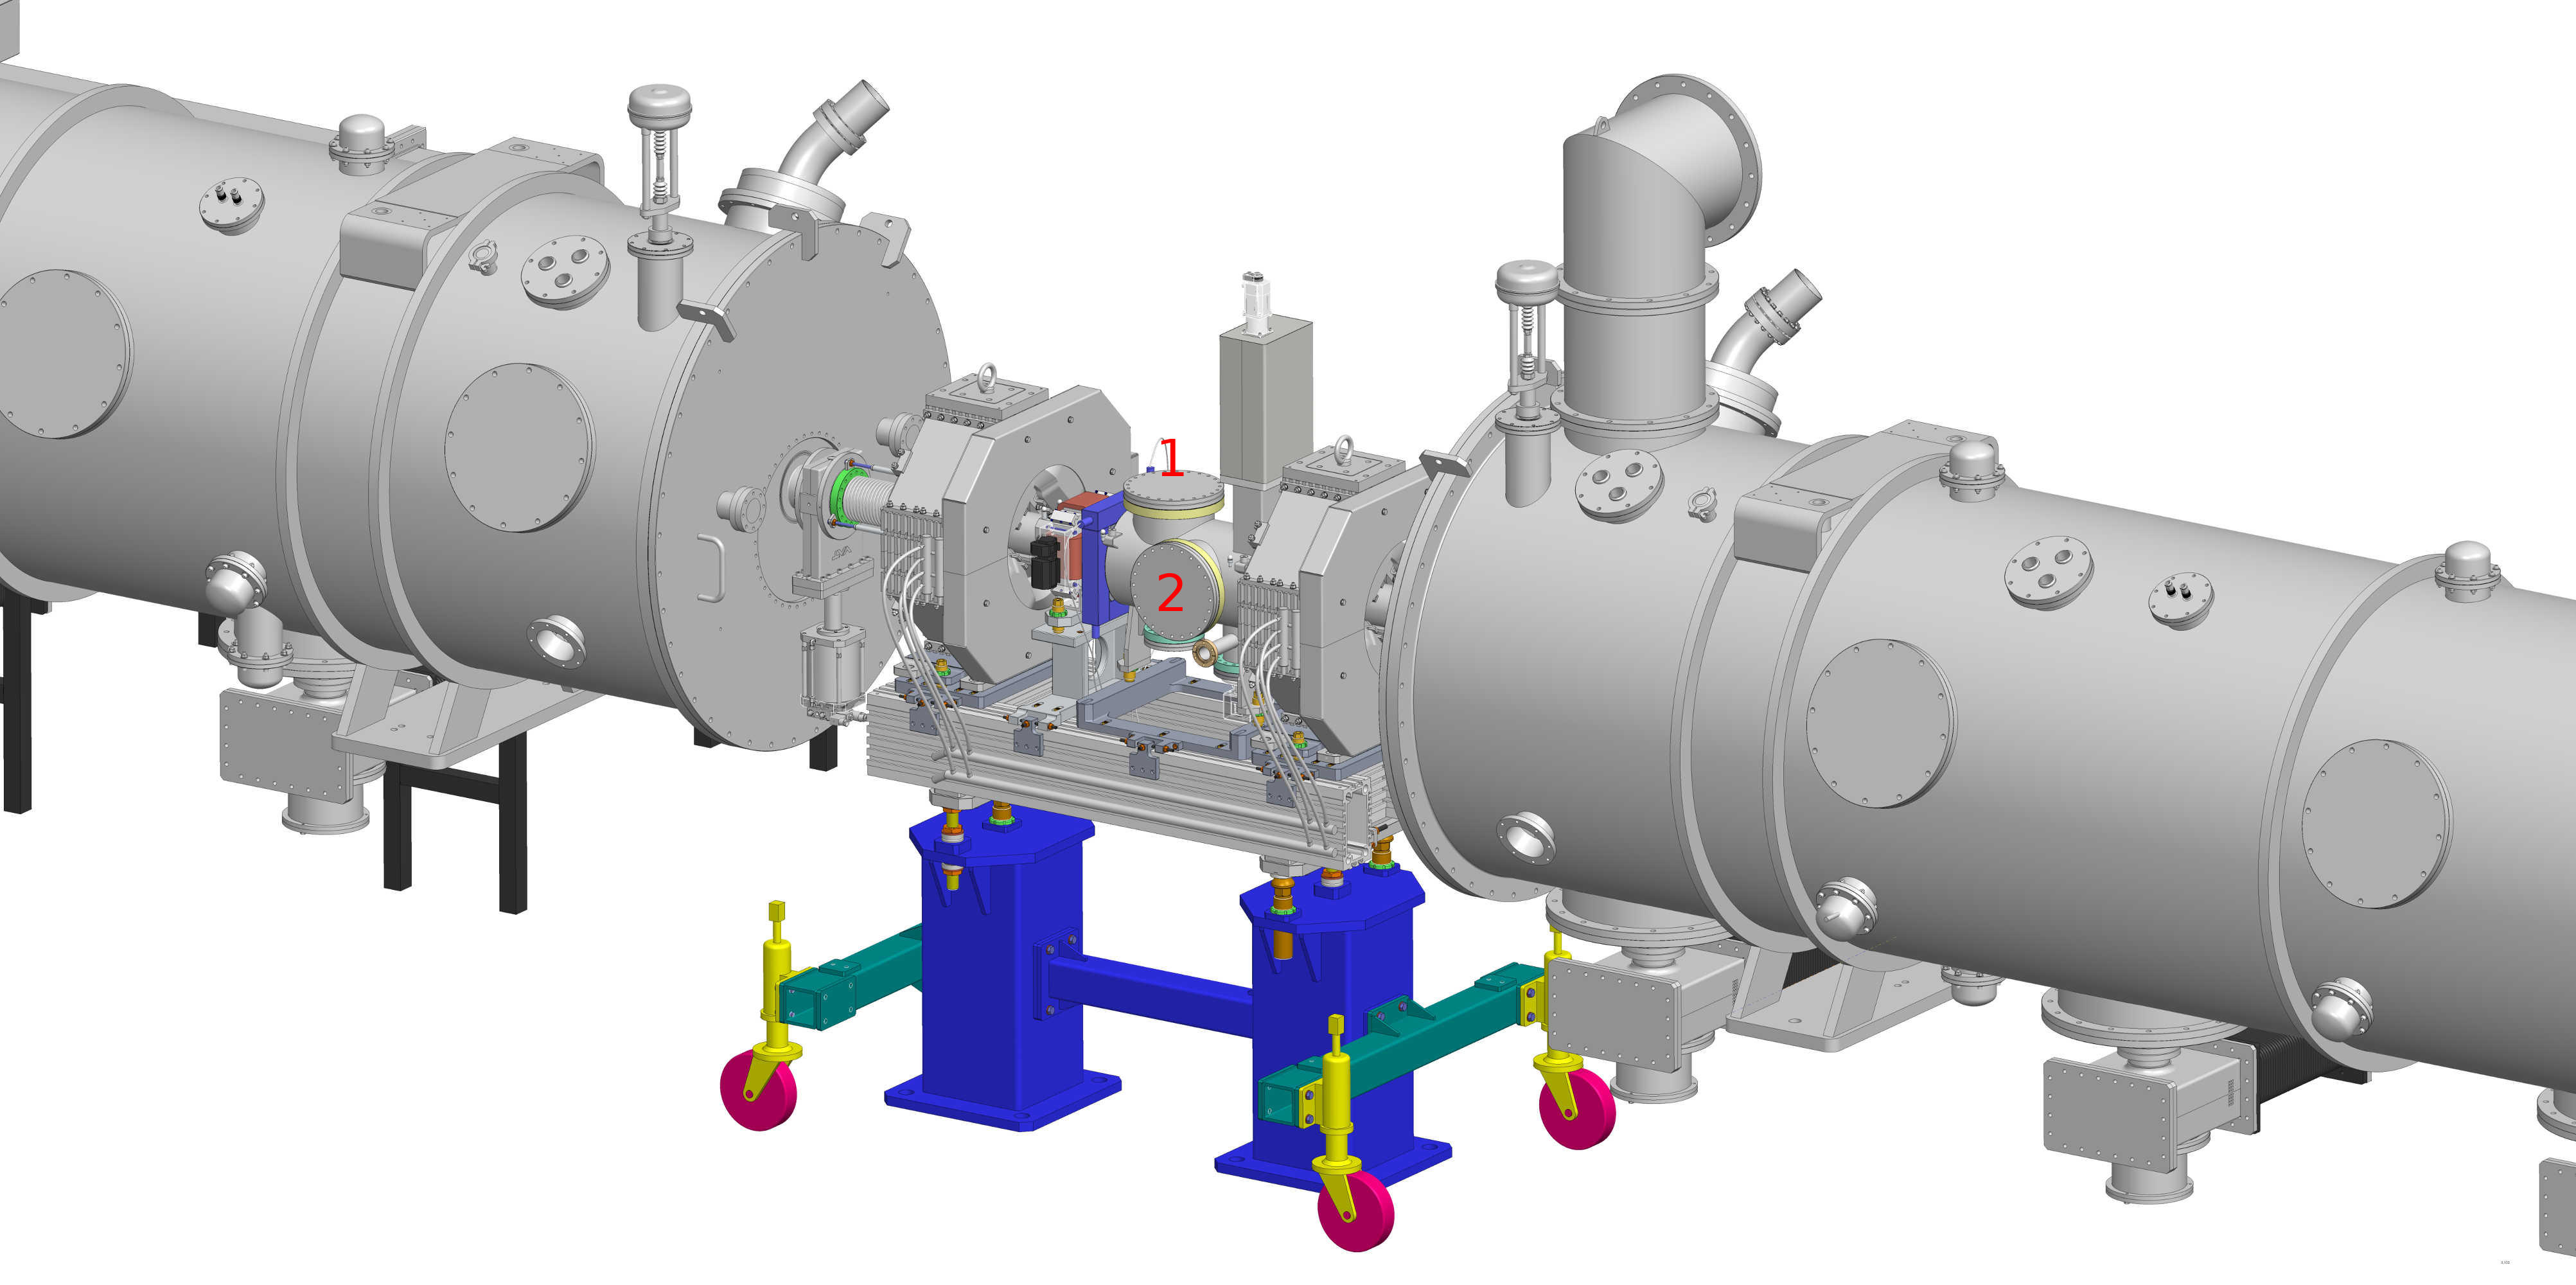
\includegraphics[width=\textwidth]{03_Prototype/figures/fig016_LWU_Cryo3.jpeg}
	\caption[The LWU vessel located between two quadrupole magnets and two cryomodules]{The LWU vessel located between two quadrupole magnets and two cryomodules. The IPMs will be mounted on the CF 200 flanges 1 and 2.}
	\label{chap3:LWU_Cryo}
\end{figure}


	The \acrshort{ipm} will be located between two cryomodules in the cold accelerator area. The \acrshort{lwu} vessels are not cooled down however the superconducting cavities are closeby. The use of superconducting cavities imposes a high vacuum and a clean environment. Indeed, a too high pressure or a contamination may damage the cavities. An operating pressure of \(10^{-9}\,\mathrm{mbar}\) is foreseen, but the vacuum level may be even lower during the operation. However, the safety valves will be closed in case of the vacuum would reach \(10^{-7}\,\mathrm{mbar}\). Hence, our \acrshort{ipm} design must be compliant with a high vacuum level and particle-free environment (ISO-5 \cite{ISO14644}). Fig. \ref{chap3:LWU_Cryo} shows the \acrshort{lwu} vessel located between two cryomodules. One can see the two \acrshort{cf} 200 flanges devoted to X and Y IPMs and the two rectangular \acrshort{cf} flanges for the X and Y wire scanners.

	\section{IPM simulations overview}

	\begin{wrapfigure}{r}{0.5\textwidth}
	\centering
	\begin{tikzpicture}%[scale=1.3]
		% Variables
		% Ipm
		\pgfmathsetmacro{\LIPM}{1.8};
		\pgfmathsetmacro{\HIPM}{1.8};
		\pgfmathsetmacro{\TIPM}{0.1};
		% Deg
		\pgfmathsetmacro{\LDEG}{0.1};
		\pgfmathsetmacro{\HDEG}{0.3};
		\pgfmathsetmacro{\NDEG}{6};
		\pgfmathsetmacro{\SDEG}{1.5};
		\pgfmathsetmacro{\SPAND}{(2*\SDEG - \HDEG)/\NDEG}

		\draw[] (\LIPM,0) node[right,align=left] {Field\\correctors\\or\\degraders};


		% Beam
		\draw[fill=blue!30] (0,0) circle (0.4) node[left,xshift = -0.3cm] {Beam};
		% Cage
		\draw (0,0) (-\LIPM,\HIPM)rectangle(\LIPM,\HIPM+\TIPM) node[above] {Anode};
		\draw (0,0) (-\LIPM,-\HIPM)rectangle(\LIPM,-\HIPM-\TIPM) node[below] {Cathode};
		\draw[fill=red!50] (-\LIPM/2,-\HIPM) rectangle(\LIPM/2,-\HIPM-\TIPM) node[midway,below] {Readout};
		% Ionized particle
		\draw[blue, dashed,->] (0.1,0.8)--(0.1,\LIPM);
		\draw[blue,fill=blue] (0.1,0.8) circle [radius=1mm] node[] {\tiny\color{white}{$-$}};

		\draw[red, dashed,->] (0.16,-1)--(0.16,-\LIPM);
		\draw[red,fill=red] (0.16,-1) circle [radius=1mm] node[] {\tiny\color{white}{$+$}};

		\draw[blue,dashed,->] (-0.1,0.1)--(-0.1,\LIPM);
		\draw[blue,fill=blue] (-0.1,0.1) circle [radius=1mm] node[] {\tiny\color{white}{$-$}};

		\draw[red,dashed,->] (-0.1,-0.1)--(-0.1,-\LIPM);
		\draw[red,fill=red] (-0.1,-0.1) circle [radius=1mm] node[] {\tiny\color{white}{$+$}};

		%Field
		\draw[->] (-1.2,1.5)--(-1.2,0.6) node [midway,right]{$\vec{E}$};
		% Degradors
		\foreach \x in {0,...,\NDEG}{
				\draw (0,0) (-\LIPM,\x*\SPAND - \SDEG) rectangle (-\LIPM+\LDEG,\x*\SPAND+\HDEG-\SDEG);
				\draw (0,0) (\LIPM,\x*\SPAND - \SDEG) rectangle (\LIPM-\LDEG,\x*\SPAND+ \HDEG-\SDEG);}


		%Profile
		\begin{axis}[every axis plot post/.append style={
						mark=none,domain=-3:3,samples=50,smooth},
				clip=false,
				axis y line=none,
				axis x line*=bottom,
				ymin=0,
				ymax=1,
				xtick=\empty,
				width=4cm,
				height=3cm,
				scale only axis,
				xshift=-2cm,
				yshift=-3.5cm
			]
			\addplot {\gauss{0}{0.3}{0.3}};
		\end{axis}

	\end{tikzpicture}
	\centering
	\caption[Visual explanation of how an IPM works]{Visual explanation of how an IPM works. The electric field between the electrodes can be reverted by inverting the polarity, making it possible to choose if detecting ions or electrons. Field correctors or degradors, left and right, improve the field uniformity.}
	\label{chap3:ipm_outline}
\end{wrapfigure}


	As explained in the previous chapter, Ionization Profile Monitor (\acrshort{ipm}) is a non-invasive detector (\acrshort{npm}) that measures the transverse profile of a beam.
	The principle of operation is summarized into three main steps (Fig. \ref{chap3:ipm_outline}):
	\begin{enumerate}
		\item Beam protons pass through the vacuum, inducing ionizations on the residual gas molecules: electron/ion pairs are created.
		\item Inside the \acrshort{ipm}, a strong electric field drives electrons or ions towards a segmented readout system.
		\item The profile is reconstructed in one transverse direction. For a complete profile, a pair of \acrshort{ipm}s, rotated by $90\textdegree{}$ to each other, is mandatory.
	\end{enumerate}

	Unfortunately, there is not a simulation software that allows a full simulation of an \acrshort{ipm}. Each step requires specific tools. In fact, most of the work consists of linking each simulation step together. The simulation can be split in the three main categories, reported just above. This chapter deals with all the simulations and approximations that has been developed to design our detector.

	We have to remind that designing IPMs to work in the requested conditions is really challenging. Preliminary studies were done in order to check the feasibility of IPM design. We focussed our reflection on the following hot topics:
	\begin{itemize}
		\item Ionization signal for ensuring that very low residual pressure and low ionization cross section at high proton energy can be manageable.
		\item The extraction field must be as uniform as possible in order to lead efficiently and correctly the ionization by-products toward the readout. %Difficulties come from the small amount of space available in the LWU.
		\item The space charge effect induced by the beam and the initial momentum of ionization electrons/ions, which may distort the profile, must be evaluated.
		\item The choice of an efficient readout technology which must match ESS working conditions.
	\end{itemize}
	All these points will be presented below.

	%  Firstly, the primary number of electron/ion pair created by the proton beam should be evaluated, and it must be sufficient in order to reconstruct a beam profile. However, this does not guaranteed that the primary particles reach the readout plane. Thus, it is necessary to perform some electromagnetic simulations. Indeed, primary particle are sensitive to the non uniformities of the extraction field and to space charge effects induced by the beam. These effects may disturb the profile measurements or reduce the number of primary particles. Therefore, they should be quantified. Lastly, the signal creation in the readout device should be evaluated with respect to previous simulations. The response of the readout mainly depends on its type.

  \section{Particle through matter}
  \label{chap3:sec_particle_in_matter}
	The interactions of particles with matter are an important aspect of particle detection \cite{Knoll2010,Leo1994}. A particle will lose energy when it passes through a medium. The physical process behind the energy transfer mainly depends on the characteristics of the particle and the medium. These topics have been studied and improved over the last century. It often combines complicated theoretical laws with approximations or empirical models. This topic is very wide, hence in the following only the pertinent information for this study will be reported.

	As explained before, the \acrshort{ipm}s rely on the by-product collection of the ionized residuals gas. The number of ionized particles gives the signal strength which has to be compliant to the readout sensitivity. Therefore, we need to know how many particles are created by the beam itself along the residual gas enclosed in the accelerator beam pipe. Then we should understand how these secondary particles create signal in the sensitive part of our \acrshort{ipm}.


	\subsection{Interaction of charged particles with matter}
	For heavy charged particles, the main interaction is due to electromagnetic interactions of the incident particle with the orbiting electrons of the medium. A particle is considered heavy if its mass is much higher than the mass of an electron. The incident particle transfers a small amount of its energy to an electron of the medium at each electronic collision. In 1930, Bethe (original paper \cite{Bethe1930}) proposed an equation that describes the mean rate of energy losses per distance unit by a heavy charged particle. The so-called Bethe equation derives from coulomb interactions. This equation has been improved over years \cite{Fermi1940,Fano1963}. The expression of the linear stopping power for heavy charged particle is defined by the following equation \cite[p. 446]{Tanabashi2018}:
	\begin{equation}
		- \bigg \langle \frac{dE}{dx} \bigg \rangle =K \rho \frac{Z}{A} \frac{z^{2}}{\beta^{2}} \left[\frac{1}{2} ln \left(\frac{2 m_{e} \beta^{2} \gamma^{2} T_{max}}{I^{2}} \right) - \beta^{2} - \frac{\delta(\beta \gamma)}{2} - \frac{C}{Z} \right]
	\end{equation}

	Where \(K\) is a constant factor defined by \(K=4 \pi N_{a} r_{e}^{2} m_{e} c^{2}\), \(r_{e}\) is the classical electron radius, \(m_{e}\) is the electron mass, \(N_{a}\) the Avogadro constant and c the speed of light in vacuum. For convenience, the stopping power is usually expressed in \(\mathrm{MeV/cm}\). In this case, \(K\) is equal to \(0.307075\).

	Terms in the Bethe equation can be dissociated in two groups. First, the incident particle related terms. The maximum transfer energy for one collision is given by the following equation:
	\begin{equation}
		T_{max} = \frac{2 m_{e} \beta^{2} \gamma^{2}}{1 + \frac{2 \gamma m_{e} }{M} + \left( \frac{m_{e}}{M} \right)^{2}}
	\end{equation}
	Where, \(M\) and \(m_{e}\) are respectively the incident particle and electron masses. The \(\beta\) and \(\gamma\) variables have their normal significance as Lorentz factors.

	Finally, the terms related to the medium. \(Z\), \(A\) and \(\rho\) are respectively the atomic number, the mass number and the density of the given medium. In most of the cases the \(\frac{Z}{A}\) ratio is close to \(0.5\) except when a medium contains hydrogen. Sometime, the Bethe equation is given independently from the density.
	The mean excitation energy \(I\) is the only non-trivial variable in the Bethe equation \cite{Berger1984,Berger1993}. The computation is quite complicated because it requires to measure the oscillator strength for each material. Table \ref{chap3:WandI} gives the \(I\) value for common materials.

	Two correction factors are often used to improve the accuracy of the Bethe equation at low and high energies. The density effect \(\frac{\delta(\beta \gamma)}{2}\) which corrects the effects at relativistic energies \cite{Sternheimer1984}. The shell correction \(\frac{C}{Z}\) improves the accuracy at low energies \cite{Bichsel2002}.

	\begin{figure}[!ht]
	\includesvg[width=\textwidth]{03_Prototype/figures/fig001_bethe_4}
	\caption[Typical mass stopping power plot a proton]{Typical mass stopping power plot for a proton. Here the mass stopping power is plotted for a proton in hydrogen and nitrogen. The calculation was done using the Bethe formula and has been cross-checked with the NIST PSTAR table which contains both computed and experimental values \cite{Seltzer1993}.}% The Bethe %equation gives correct results between \(0.2\ <\ \beta\gamma\ <\ 100\). %However at lower and higher energies the Bethe formula is no more reliable.}
	\label{chap3:bethe1}
\end{figure}


	Fig. \ref{chap3:bethe1} shows the mass stopping power of a proton in two different mediums. The blue region represents the energy range of protons in the cryogenic part of \acrshort{ess}, where \acrshort{ipm}s will be located. One can see that the minimum of energy loss is reached around \(2\,\mathrm{GeV}\).

	The Bethe model has been tested and improved with respect to experimental data \cite{Porter1990}. However, at very low or high energies the Bethe equation is no more usable. In these regions specific models are used to describe the energy loss in matter \cite{Ziegler1985, Allison1980}.

	The Bethe model is also not compatible with low mass particles like electrons and positrons. The Bethe formula must be modified for these particles \cite{Rieke1972}\cite[p. 452]{Tanabashi2018}. At low energies, electrons lose its energy by ionization like ions, whereas at energies above few \(\mathrm{MeV}\), electrons also lose energy through bremsstrahlung radiation.

	\subsection{Electron ion pairs production}
	We just defined the mean energy loss rate of a charged particle per unit of distance. When a particle passes through a medium it may deposit its energy to an electron of the medium (atoms).
	If the energy is sufficient, an ionization happens: an electron is ejected from the electronic shell leading to the creation of an ion and an electron in most of the case. In case of molecule, the ionization process may be dissociative i.e. it may break the molecular bound. The cross section for dissociative ionization is far lower than the one for pure ionization \cite{Dimopoulou2004}.

	By introducing \(W\), the average energy for producing an ion/electron pair in a medium, we can estimate the number of ion/electron pairs created for a given readout length \cite[]{Weiss1955,Bichsel1979}.

	\begin{equation}
		N_{electrons}= \frac{\big \langle \frac{dE}{dx} \big \rangle}{W_{n}} \Delta x
	\end{equation}

	When an electron is ejected, it has a certain probability for ionizing other atoms when its energy is high enough. These secondary electrons are called delta rays or delta electrons. This phenomenon becomes rare and negligible when the medium has a very low density like in a vacuum system. The \(W\) parameter includes the delta ray electrons, hence the \(W\) value is biased for us since our detectors work at very low pressure \cite[p. 470]{Tanabashi2018}. Table \ref{chap3:WandI} gives, as an example, the \(W\) values for several materials at Normal Temperature and Pressure\footnote{$20\,\mathrm{°C}$, $1\,\mathrm{atm}$} (NTP).

	\begin{table}[ht]
	\centering
	\caption[Mean excitation energie, average energy to produce a pair and density values for severals mediums at Normal Temperature and Pressure (NTP)]
	{Mean excitation energie, average energy to produce a pair and density values for severals mediums at Normal Temperature and Pressure (NTP). Complete reviews of \(I\) and \(W\) values are available in \cite{Kamakura2006}\cite{Bichsel1979}.}
	\label{chap3:WandI}
	\begin{tabular}{llll}
		\toprule
		Gas        & \(I\) (\(\mathrm{eV}\)) & \(W\) (\(\mathrm{eV}\)) & \(\rho\) (\(\mathrm{kg/m^{3}}\)) \\
		\midrule
		\(H_{2}\)  & \(18.8\)       & \(36.43\)  &  \(0.0899\)  \\
		\(CO\)     & \(85.9\)       & \(34.5\)   &  \(1.165\)  \\
		\(CO_{2}\) & \(85.00\)      & \(34.21\)  &  \(1.842\)  \\
		\(N_{2}\)  & \(82.00\)      & \(36.39\)  &  \(1.165\)  \\
		\bottomrule
	\end{tabular}
\end{table}

	When the medium is a mixture of several compounds then it is necessary to calculate the mean stopping power for each of them weighted by their mass proportions:
	\begin{equation}
		N_{total}= \sum_{n= First}^{Last} N_{compound\ n}= \sum_{n= First}^{Last} w_{n} \frac{\big \langle \frac{dE}{dx}\left(\rho_{n},I_{n},A_{n},Z_{n}\right) \big \rangle}{W_{n}} \Delta x
	\end{equation}
	The calculation can be done for each single element or for each molecule in the compound.
	This latter is recommended since the \(I\) values are in general higher for molecules \cite[p. 451]{Tanabashi2018}.

	\subsection{Calculation}

	Now that we have defined all the physics background, we should be able to estimate the number of primary particles that will be created in the \acrshort{ess} conditions. We tried two different approaches: naive computation of Bethe equation and simulations through a software.

	The Bethe formula is easy to implement since it requires to know only the composition of the medium and the \(I\) value of each compound. The expected pressure in the cryogenic part at \acrshort{ess} is around \(10^{-9}\,\mathrm{mbar}\), and the gas composition is given in Table \ref{chap3:ess_vacuum_gas}.

	\begin{table}[ht]
	\centering
	\caption[Expected residual vacuum gas in the cold part of ESS Linac, provided by ESS vacuum group]
	{Expected residual vacuum gas in the cold part of ESS Linac, provided by ESS vacuum group.}
	\label{chap3:ess_vacuum_gas}
	\begin{tabular}{llll}
		\toprule
		Gas        & Mass percentage (\(\%)\) & $p_{i}$ (\(\mathrm{mbar}\)) & $\rho_{i}$ $(\mathrm{g/cm^{3}}$) \\
		\midrule
		\(H_{2}\)  & \(79\)          & \(7.9 10^{-10}\)   & \(6.52\cdot
		10^{-17}\)                                                                \\
		\(CO\)     & \(10\)          & \(1.0 10^{-10}\)   & \(1.15\cdot
		10^{-16}\)                                                                \\
		\(CO_{2}\) & \(10\)          & \(1.0 10^{-10}\)   & \(1.8\cdot
		10^{-16}\)                                                                \\
		\(N_{2}\)  & \(1\)           & \(1 10^{-11}\)     & \(1.14\cdot
		10^{-17}\)                                                                \\
		\bottomrule
	\end{tabular}
\end{table}

	We assume that the residual gas follows the "perfect gas" law. We also assume that the linear density scaling of Bethe equation remains true in high vacuum \cite[p. 108]{egber2012}\cite{Ishimaru1995}. Hence, the partial pressure and the density for each gas is calculated with respect to the tabulated pressures. The primary signal is computed at \acrshort{ess} nominal conditions given in Table \ref{chap2:ess_charac}.

	Fig. \ref{chap3:ess_primary_particles} shows the number of electron ion pairs created for each gas species versus the \acrshort{ess} range of energies. The different \acrshort{ipm}s locations are marked by a blue line. One can see that the gas density has a strong influence on the primary signal. Although the hydrogen is the main species in term of proportion, its contribution to primary signal is close to the one from carbonate species. Note that the \(W\) value may overestimate the number of pairs created due to secondary delta rays.

	\begin{figure}[!ht]
	\includesvg[width=\textwidth]{03_Prototype/figures/fig015_ess_primary_particle}
	\caption[Expected number of electron/ion pairs per centimeter at ESS nominal conditions according to Bethe equation]{Expected number of electron/ion pairs per centimeter at ESS nominal conditions according to Bethe equation. Each vertical line corresponds to an IPM location.}
	\label{chap3:ess_primary_particles}
\end{figure}


	We have also used Garfield++ software to compute the number of primary particles. This software is normally intended to the gaseous detectors modelization. It allows to simulate the creation of electron/ion pairs due to the ionization of gas by an incident particle, the transport and the amplification of these electrons in the gas and the induced signal on a readout plane. In our case, we simulated only the pair creation in gas. For this step Garfield++ uses two programs internally:
	\begin{itemize}
		\item Magboltz: a Fortran routine that compute different properties of a gas mixture and the transport of electrons in this mixture \cite{Biagi1989}.
		\item Heed ++: a C ++ library that implements an ionization model based on the photoabsorption ionization (PAI) \cite{Allison1980,Smirnov2005}.
	\end{itemize}

	\begin{table}[ht]%{r}{0.5\textwidth}
	\centering
	\caption[Comparison of expected number of electrons between calculation using Bethe equation and results from Garfield++.]
	{Comparison of expected number of electrons between calculation using Bethe equation and results from Garfield++}
	\label{chap3:GarfieldBethe}
	\begin{tabular}{llll}
		\toprule
		Energy    & \(N_{Bethe}\) & \(N_{garfield}\) & Factor \\
		\midrule
		\(97.2\)  & \(100210\)    & \(52537\)             & \(0.52\)   \\
		\(231.4\) & \(54970\)     & \(27463\)             & \(0.50\)   \\
		\(278.9\) & \(49160\)     & \(26124\)             & \(0.53\)   \\
		\(315.8\) & \(45850\)     & \(23769\)             & \(0.52\)   \\
		\(628.3\) & \(33600\)     & \(17522\)             & \(0.52\)   \\
		\bottomrule
	\end{tabular}
\end{table}
	A dummy detector, a cube of ten centimeter, is implemented and filled with the same gas composition as the ESS residual gas. Then, we shoot protons into this detector. The information on the electrons created in gas is saved in a ROOT file and then processed \cite{Brun1997,Antcheva2009}. This is done for different proton energies and vacuum levels.

	The Table \ref{chap3:GarfieldBethe} reports the value of expected number of electrons/ions pairs per cm for the direct calculation from Bethe equation and results from Garfield++ simulations. One can see that the Garfield value is always lower than the calculation by a constant factor X.


	\subsection{Pressure uniformity}

	The primary signal is strongly dependant to the pressure inside the vacuum chamber. A gradient in the pressure may cause a change in the signal shape. It could be interesting to simulate the vacuum to check the existence of this kind of gradient in vacuum.

	\begin{wrapfigure}{r}{0.5\textwidth}
  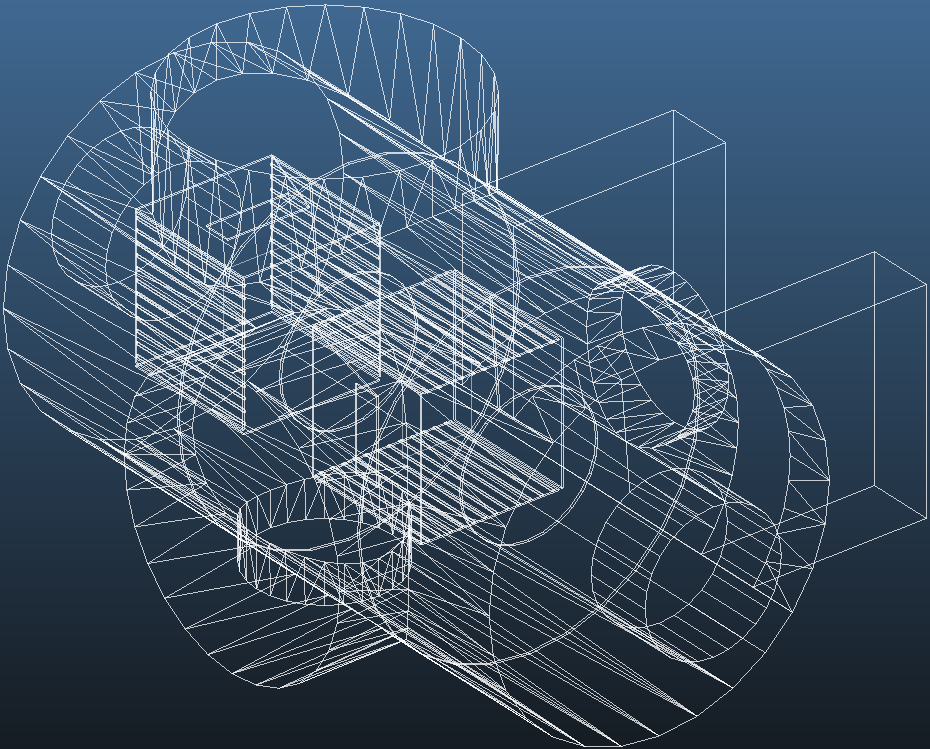
\includegraphics[width=0.5\textwidth]{03_Prototype/figures/fig019_molflow_LWU.png}
  \caption[The LWU geometry implemented in Molflow+]{The LWU geometry implemented in Molflow+.}    
	\label{chap3:molflow_LWU}
\end{wrapfigure}


	A simulation has be done with the Molflow+ software developed at CERN \cite{Kersevan2009}. It simulates the vacuum in a steady state by using Monte Carlo and Ray Tracing methods. The user defines his geometry, the desorption and adsorption rates of each surface. The geometry used is visible in Fig. \ref{chap3:molflow_LWU}. Hence, it does not contain all the structures and surfaces. Two dummy squares facets of $5\,\mathrm{cm}$ are inserted in the center of each \acrshort{ipm}. The pressure profiles are then measured on these facets. We have no information about pumping groups, surface conditions or other vacuum characteristics. Therefore, the simulation is not done for determining the vacuum achievable by our system in the LWU but to verify the uniformity of the pressure profile in both \acrshort{ipm}s. We also checked the case of a unwanted outgassing occurs on one side of the IPMs. No significant change has been observed.

	\begin{figure}[!h]
	\begin{center}
		\includesvg[width=\textwidth]{03_Prototype/figures/fig020_profile_pressure}
	\end{center}
	\caption[Simulated profile pressure in the center of IPMs.]{Simulated profile pressure in the center of IPMs.}
	\label{chap3:profile_pressure}
\end{figure}


	Fig. \ref{chap3:profile_pressure} shows results from simulations. Fortunately, pressures seem uniform along the transversal direction for two IPMs. The pressure is slightly lower in the second IPM because the pumping group is closer. However, this may not affect the profile measurement.

	\section{Extraction field}
	\begin{wrapfigure}{r}{0.5\textwidth}
	\centering
	\begin{tikzpicture}
		% Variables
		% Ipm
		\pgfmathsetmacro{\LIPM}{1.8};
		\pgfmathsetmacro{\HIPM}{1.8};
		\pgfmathsetmacro{\TIPM}{0.1};
		% Deg
		\pgfmathsetmacro{\LDEG}{0.1};
		\pgfmathsetmacro{\HDEG}{0.3};
		\pgfmathsetmacro{\NDEG}{6};
		\pgfmathsetmacro{\SDEG}{1.5};
		\pgfmathsetmacro{\SPAND}{(2*\SDEG - \HDEG)/\NDEG}

		% Beam
		\draw[fill=blue!30] (0,0) circle (0.4) node[left,xshift = -0.3cm] {Beam};
		% Cage
		\draw (0,0) (-\LIPM,\HIPM)rectangle(\LIPM,\HIPM+\TIPM) node[above] {Anode};
		\draw (0,0) (-\LIPM,-\HIPM)rectangle(\LIPM,-\HIPM-\TIPM) node[below] {Cathode};
		\draw[fill=red!50] (-\LIPM/2,-\HIPM) rectangle(\LIPM/2,-\HIPM-\TIPM) node[midway,below] {Readout};
		% Ionized particle
		\draw[blue, dashed,->] (0.1,0.8)to [bend right=15](-0.1,\LIPM);
		\draw[blue,fill=blue] (0.1,0.8) circle [radius=1mm] node[] {\tiny\color{white}{$-$}};

		\draw[red, dashed,->] (0.36,-1)to [bend left=0](0.56,-\LIPM);
		\draw[red,fill=red] (0.36,-1) circle [radius=1mm] node[] {\tiny\color{white}{$+$}};

		\draw[blue,dashed,->] (-0.1,0.1)to [bend right=15](-0.8,\LIPM);
		\draw[blue,fill=blue] (-0.1,0.1) circle [radius=1mm] node[] {\tiny\color{white}{$-$}};

		\draw[red,dashed,->] (-0.1,-0.1)to [bend right=15](0.2,-\LIPM);
		\draw[red,fill=red] (-0.1,-0.1) circle [radius=1mm] node[] {\tiny\color{white}{$+$}};

		%Field
		\draw[->] (-1.2,1.5)--(-1,0.6) node [midway,right]{$\vec{E}$};

		% Profile
		\begin{axis}[every axis plot post/.append style={
						mark=none,domain=-3:3,samples=50,smooth},
				clip=false,
				axis y line=none,
				axis x line*=bottom,
				ymin=0,
				ymax=1,
				xtick=\empty,
				width=4cm,
				height=3cm,
				scale only axis,
				xshift=-2cm,
				yshift=-3.5cm
			]
			\addplot {\gauss{0.75}{0.5}{0.3}};
		\end{axis}
	\end{tikzpicture}
	\centering
	\caption[Non-uniformities leading to mirage effects on the profile measurement]{Non-uniformities leading to mirage effects on the profile measurement.}
	\label{chap3:FieldNonU_outline}
\end{wrapfigure}

	The \acrshort{ipm}s can be seen as a parallel plate detector. In an ideal \acrshort{ipm} these plates are infinite sized. The extraction field is then completely oriented in a single direction, normal to the detection plane. So the projection of the profile is perfect on this plane. In reality, the plates can not be considered infinite sized with respect to the gap between the two electrodes. In these conditions the field is no more uniform for several reasons.

	The effects induced by the cage sides are no longer negligible; field uniformity is strongly influenced by the needle effects of the plates.
	Also, the geometry of the vacuum chamber has also some influences on the field uniformity. Indeed the vacuum chamber is considered to be at ground. Walls close to the \acrshort{ipm}s will change the electric field lines inside the \acrshort{ipm}s. As well, the cross-interaction between two IPMs close by is very strong in limited space environnement.

	Finally, the way to create the field with high voltage (\acrshort{hv}) power supplies has a important influence on the field. We will see later that some readouts can only work in certain configurations of high voltages.

	The non-uniformity of the electric field is very problematic because it creates mirage effects and prevents the correct measurement of the beam profile as shown in Fig. \ref{chap3:FieldNonU_outline}. It also determines the maximum size of the detection area which must be in a zone as uniform as possible. To overcome all these effects, the field line must be straight as possible. Several solutions can be considered to improve the field uniformity:
	\begin{itemize}
		\item The distance between the two electrodes for a same electrode size. In same way, the size of both electrodes can be increased. In this case, the \acrshort{ipm}s will tend to a configuration close to the infinite parallel plates assumption. However, these solution are mainly limited due to mechanical considerations. The whole assembly of one \acrshort{ipm} must fit on a CF 200 flange.
		\item The field uniformity can be improved by the use of field correctors or field degraders \cite[p. 103]{egber2012}. This is done by placing conductors on each side. Correctors are polarized at a certain potential in order to constraint the field. This solution is easy to implement, compact, and very versatile. However, it requires a large number of \acrshort{hv} feedthroughs or the use of resistors in vacuum. The longitudinal field can also slightly improved in a same way.
		\item To protect against the \acrshort{ipm} cross-interaction, one can put grounded conductors between the two \acrshort{ipm}s \cite[p. 132]{egber2012}. The cross interaction are also reduced with longitudinal correctors.
		\item The geometry of \acrshort{hv} electrodes. For example, a curved geometry with reinforcements on the edges it is possible to correct the field transversely and longitudinally \cite{Bartkoski2014}. Hence, there is no more need of field correctors. On the other hand, the electrode is generally larger electrode and optimized for a precise configuration.
		\item Lastly, software corrections may be a solution to correct the non uniformities. However, the non-uniformity of extraction field is not the only phenomenon responsible of the profile distortions as explained previously. It is therefore extremely difficult to implement and requires a perfect map of the extraction field to decouple it from other phenomena. Physical corrections are then much simpler to implement.
	\end{itemize}

  % The second limitation concerns possible \acrshort{hv} breakdowns. In very high vacuum a distance of some millimeter is sufficient to isolate several tens of kilovolts. However, the breakdowns are also strongly influenced by the surface states of the electrodes, the composition of the vacuum and the presence of leakage current \cite{Latham1995}. Hence, we should keep a standoff distance between the electrode and the vacuum vessel (less than 1kV/cm between the IPMs and LWU).

	\subsection{Maxwell equations at steady state}
	Electric and magnetic fields are perfectly described by the Maxwell's equations. Since we are in a vacuum, so the Maxwell's equations can be reduced to:
	\begin{alignat*}{3}
		\overrightarrow{\nabla} \cdot \overrightarrow{E}  & = \frac{\rho}{\epsilon_{0}}\quad                                           &  & \text{(Maxwell-Gauss's Law)}   \\
		\overrightarrow{\nabla} \times \overrightarrow{E} & = - \frac{\partial \overrightarrow{B}}{\partial t}\quad                    &  & \text{(Maxwell-Faraday's Law)} \\
		\overrightarrow{\nabla} \cdot \overrightarrow{B}  & = 0\quad                                                                   &  & \text{(Maxwell-Thomson's Law)} \\
		\overrightarrow{\nabla} \times \overrightarrow{B} & = \overrightarrow{J} + \frac{\partial \overrightarrow{E}}{\partial t}\quad &  & \text{(Maxwell-Ampère's Law)}
	\end{alignat*}

	The time derivatives cancel each other, when the field variations over time are negligible compare to the studied phenomena. So, the coupling effects between the electric and the magnetic fields disappear. Therefore, the electrostatic field depends only on the Gauss’s law. In electrostatic, it is quite convenient to introduce the electric potential:
	\begin{equation}
		\vec{E} = - \vec{\nabla}V
	\end{equation}

	\subsection{Solving Poisson's equation}
	The electric potential follows a Poisson's equation:
	\begin{align}
		 & \Delta V = \vec{\nabla}^{2}V = -\frac{\rho}{\epsilon_{0}} \\
		 & \Delta v = f
	\end{align}

	The solution of this equation can be found analytically. These methods mainly rely on the use of complex numbers or Laplace transforms. However, when the size of the problem increases the solution becomes harder to compute, and solving the Poisson's equation on complicated domains is almost impossible. The numerical methods allow to approximate the solutions of partial differential equations (\acrshort{pde}) on complex domains. There are many schemes to solve numerically \acrshort{pde}. In this section we will briefly present three methods that are often used. It is important to understand how they work and to know their limitations or pitfalls. In numerical schemes, the domain is discretized in a finite set of points. Then, the solution is approximated at each point with respect to initial and/or boundary conditions. To solve a problem, it must be well posed: the problem must admit a single unique solution that depends continuously on the variables and conditions \cite{Hadamard1902}. It turns out that the Poisson's equation is a well-posed problem if a Dirichlet condition is applied.

	\paragraph{}
	Finite Difference Method (FDM) is a popular way to solve numerically the Poisson’s equation. In FDM, the domain is discretized regularly with a step h. The Taylor's theorem allows to approximate the value of a function by a polynomial equation that depends on its derivatives nearby:
	\begin{align}
		 & v(x+h) = v(x)+hv^{\prime}(x)
		+\frac{h^2}{2}v^{\prime\prime}(x)+\frac{h^3}{6}v^{\prime\prime\prime}(x) + O(h^{4}) \\
		 & v(x-h) = v(x)-hv^{\prime}(x)
		+\frac{h^2}{2}v^{\prime\prime}(x)-\frac{h^3}{6}v^{\prime\prime\prime}(x) + O(h^{4})
	\end{align}
	From these formulas, the second derivative can be expressed and in case of a two-dimensional domain it is written as follows:
	\begin{equation}
		\begin{split}
			h^{2}v^{\prime\prime}(x,y)=&v(x+h,y) + v(x-h,y) \\
			+ &v(x,y+h) + v(x,y-h) \\
			- 4&v(x)+ O(h^{2})
		\end{split}
	\end{equation}
	Each point of the domain can be expressed according to its neighbors. Then, it is possible to write a set of linear equations in matrix form by choosing wisely the indexing order. For example, when the domain is decomposed line by line, one can obtain the same system of equations repeated for each inner line \footnote{The first and last lines have a slightly different set of equations.}.
	\begin{equation}
		Id \cdot v_{u} + A \cdot v_{c} + Id \cdot v_{d} = D
	\end{equation}
	Where $ A =
		\begin{pmatrix}
			-4     & 1      & 0      & \cdots \\
			1      & -4     & 1      & \cdots \\
			0      & 1      & -4     & \cdots \\
			\vdots & \vdots & \vdots & \ddots
		\end{pmatrix} $ is the square matrix of FDM schemes, $v$ is the unknown value vector and $D$ is vector of Dirichlet values. Then, the global matrix is assembled by combining the sub-matrices for each line.
	\begin{equation}
		\begin{bmatrix}
			A      & Id     & 0      & \cdots \\
			Id     & A      & Id     & \cdots \\
			0      & Id     & A      & \cdots \\
			\vdots & \vdots & \vdots & \ddots
		\end{bmatrix}
		\cdot
		\begin{bmatrix}
			v \\
			v \\
			v \\
			\cdots
		\end{bmatrix}
		=
		\begin{bmatrix}
			D \\
			D \\
			D \\
			\cdots
		\end{bmatrix}
	\end{equation}
	On can see that the problem is solved by inverting the A matrix. This matrix is very sparse and can be inverted with iterative methods rather than a direct inversion. FDM is straightforward and allows to quickly solve Poisson’s equation on a linear structured mesh. For instance, it is very useful for calculating an electric field generated by a charge density. However, FDM cannot be used when the geometry becomes too complex.

	\paragraph{}
	The Finite Element Method (FEM) is more suitable for solving PDE on complex domains. The FEM uses the weak formulation of the Poisson’s equation. By introducing a test function $\varphi$, this weak form can be written easily thanks to an integration by parts:
	\begin{align}
		\int_{\Omega}^{} \varphi \Delta v d\Omega                                                                                     & = \int_{\Omega}^{} \varphi f d\Omega                                                            \\
		\int_{\Omega}^{} \vec{\nabla} \varphi \cdot \vec{\nabla} v d\Omega - \int_{d\Omega}^{} \varphi \vec{\nabla} v \cdot n d\Sigma & = \int_{\Omega}^{} \varphi f d\Omega                                                            \\
		\int_{\Omega}^{} \vec{\nabla} \varphi \cdot \vec{\nabla} v d\Omega                                                            & = \int_{\Omega}^{} \varphi f d\Omega + \int_{d\Omega}^{} \varphi \vec{\nabla} v \cdot n d\Sigma
	\end{align}
	One can see that the Laplacian disappeared from the formulation. An approximation of $v$ is done in the reduced domain by the mean of low order polynomial functions. Again, a finite system of linear equations can be written, and the problem is solved by inverting the matrix. The correct choice of test functions and the way to index elements lead to very sparse matrix which can be inverted easily. Unlike the FDM, the solution is approximated on the whole reduced domain and not locally. FEM supports complex meshes as long as they are continuous and solves all kinds of PDEs that may be much more complex than the Poisson’s equation.

	\paragraph{}
	% Expliquer mieux les BEM
	With FEM, the whole domain is fully discretized and. In the case of electrostatic, it is possible to use the Boundary Element Method (BEM). With the BEM, the Poisson’s equation is first solved on boundaries. Then, the electric field can be evaluated at any point in the domain from the contributions of all boundaries. The discretization is also performed only on the boundaries and not on the entire geometry. So, the dimension of the problem is reduced and the matrix to be reversed is then much smaller. On the other hand, the matrix is ​​no longer sparse.

	Most of the commercial simulation softwares rely on FEM or BEM \cite{cststudio2018,ansys2018,couloumb2018}. We have used mainly COMSOL software for the simulations of extraction field.

	\subsection{COMSOL}
	COMSOL is commercial all-in-one multi-physics simulation software able to solve various problems from structural mechanical analysis to optical raytracing \cite{comsol2018}. We use COMSOL with the AC/DC module to simulate the static electric field in the \acrshort{ipm} box \cite{comsolacdc2018}. COMSOL allows to quickly define, simulate and post process physical model. The typical workflow is divided in three main steps as follow.

	\paragraph{}
	The first step is to implement the detector geometry into COMSOL. The software includes basic \acrshort{cad} features allowing to quickly create two or tridimensional geometries. The users can directly import a mesh from file generated by external \acrshort{cad} tools. Care should be taken from importing \acrshort{cad} file, it often contains many details and thus increase the CPU time consumption. It is much faster to directly implement the geometry with COMSOL.  In our case, only the inner shape of the vacuum chamber and the \acrshort{ipm}s must be defined. All other conductive bodies that enclose the vacuum are not relevant for an electrostatic simulation. Therefore, the geometry can be simplified. Fig. \ref{chap3:COMSOL_LWU} shows, on the left, a 3D drawing of the \acrshort{ess} vacuum vessel with the two \acrshort{ipm}s inside. And on the right, an example of the simplified geometry implemented in COMSOL.

	\begin{figure}[ht]
	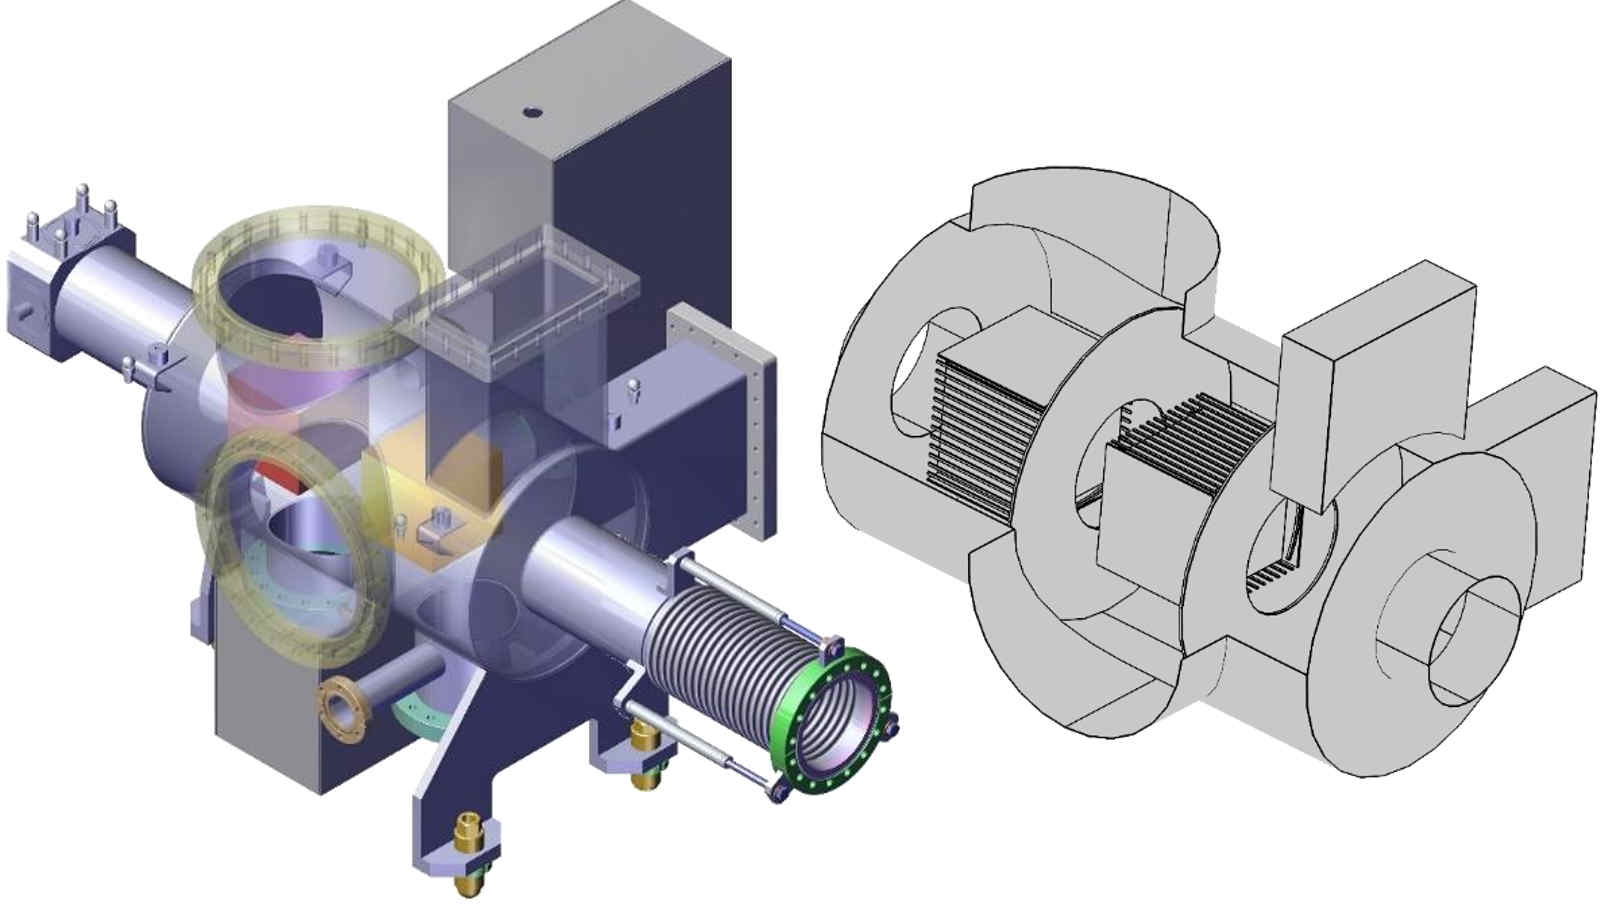
\includegraphics[width=\textwidth]{03_Prototype/figures/fig003_COMSOL_LWU.jpeg}
	\caption[A drawing of LWU (left) and its implementation in COMSOL (right)]{A drawing of LWU (left) and its implementation in COMSOL (right).}
	\label{chap3:COMSOL_LWU}
\end{figure}


	\paragraph{}
	The next step consists on the discretization of the previous geometry in many Lagrange elements in order to form a mesh. Fig. \ref{chap3:COMSOL_meshing_elements} shows the main meshing elements available in COMSOL. For an electrostatic tri-dimensional study, COMSOL uses quadratic tetrahedral elements by default. The meshing algorithm tries to create elements fitting well the geometry. For the inner small parts of the geometry, the size of elements will be reduced in these regions. Conversely, mesh cells will become bigger and bigger in coarse regions of the geometry. This behavior is not desirable for us, since the \acrshort{ipm} region of interest has no geometrical variation. Thus, the geometry will be not described accurately. Fortunately, the user can change the characteristics and the nature of the elements in specific region of the defined geometry. We used a tetrahedral mesh apart from the \acrshort{ipm} box where a cubic mesh with high granularity is defined. The meshing step is very memory consuming, but a poorly optimized mesh may destroy performance.

	\begin{figure}[ht]
	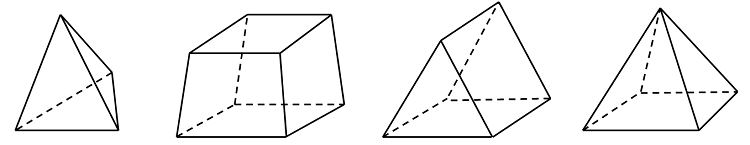
\includegraphics[width=\textwidth]{03_Prototype/figures/fig006_COMSOL_meshing_elements.png}
	\caption[3D Mesh elements included in COMSOL]{Mesh elements included in COMSOL software. From left to right: tetrahedron, hexahedron, prism and pyramid \cite{mesh2013}. COMSOL uses tetrahedral elements by default to mesh a 3D geometry in AC/DC module.}
	\label{chap3:COMSOL_meshing_elements}
\end{figure}


	\paragraph{}
	The last step is to define boundary conditions. COMSOL hides completely the mathematical aspect of the \acrshort{fem}/\acrshort{bem} and directly express the boundary conditions in a physical meaning. In case of the AC/DC module, this means that the user should fix potentials or charge densities on boundaries. A more detailed description of each boundary condition type can be found in the reference manual. COMSOL is able to solve electrostatic problems by means of \acrshort{fem} or \acrshort{bem} since version 5.3a. We compared the \acrshort{fem} and \acrshort{bem} for same configurations and we found out that results are slightly different as shown in Fig. \ref{chap3:FEMvsBEM}. We decided to use mainly \acrshort{fem} since it is the legacy method in COMSOL.
	Once solved, the problem can be processed directly in COMSOL. Data can be also exported to an external file in text format (column separated values or VTU format).

	\begin{figure}[!h]
	\begin{subfigure}{.5\textwidth}
		\centering
		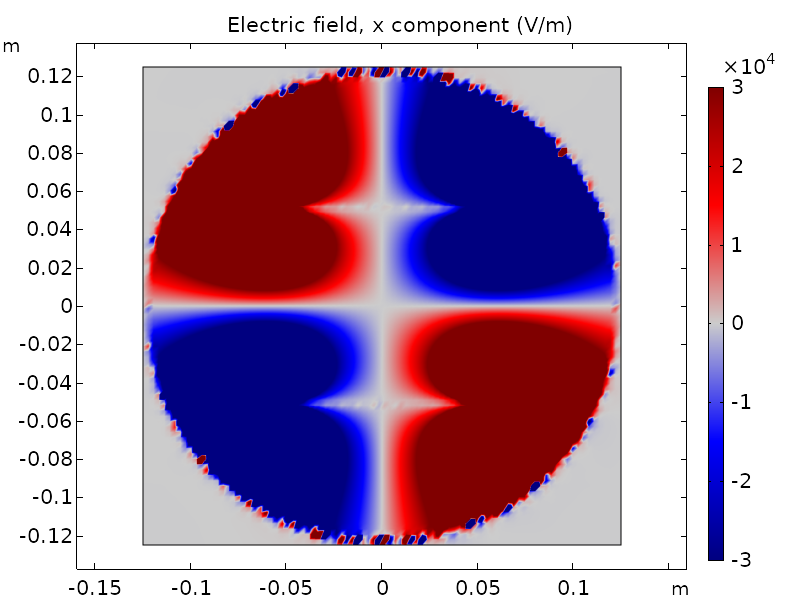
\includegraphics[width=\textwidth]{03_Prototype/figures/fig012_BEMa.png}
		\caption{Configuration 1 solved with BEM.}
		\label{}
	\end{subfigure}\hfill
	\begin{subfigure}{.5\textwidth}
		\centering
		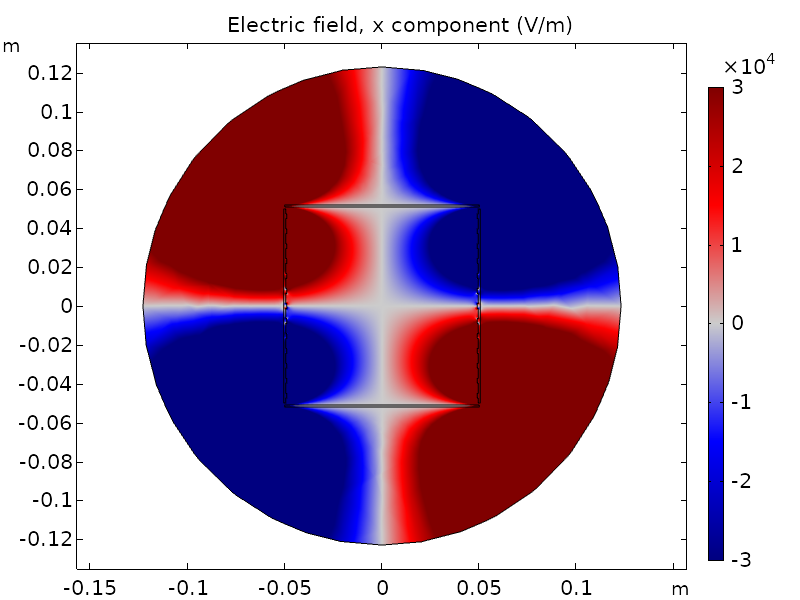
\includegraphics[width=\textwidth]{03_Prototype/figures/fig012_FEMa.png}
		\caption{Configuration 1 solved with FEM.}
		\label{}
	\end{subfigure}
	\vskip\baselineskip
	\begin{subfigure}{.5\textwidth}
		\centering
		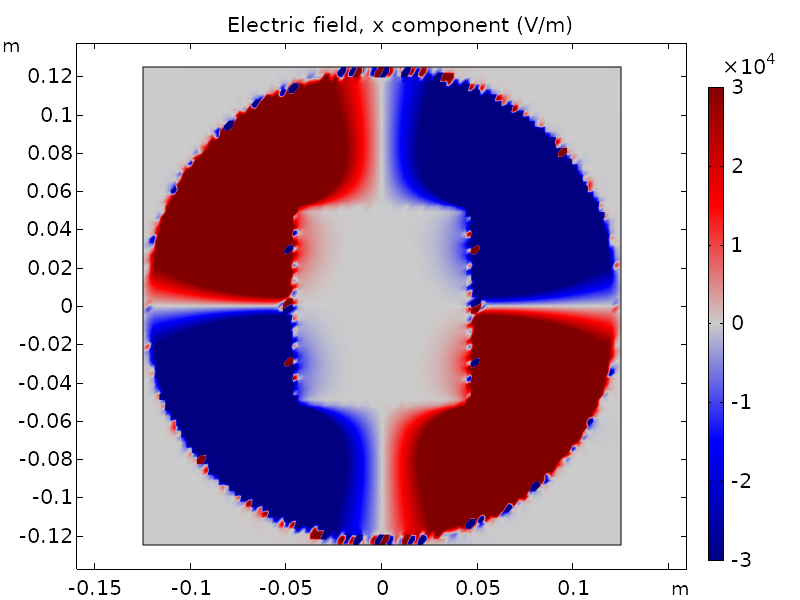
\includegraphics[width=\textwidth]{03_Prototype/figures/fig012_BEMb.png}
		\caption{Configuration 2 solved with BEM.}
		\label{}
	\end{subfigure}\hfill
	\begin{subfigure}{.5\textwidth}
		\centering
		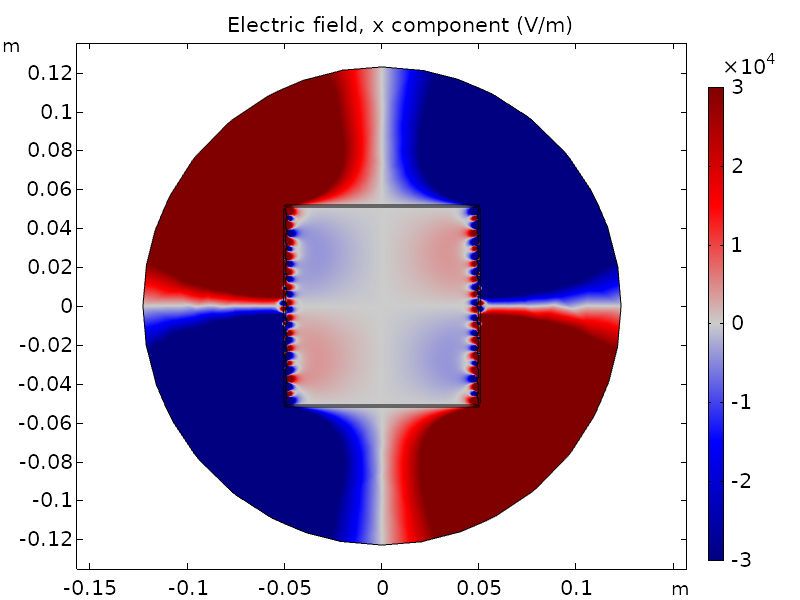
\includegraphics[width=\textwidth]{03_Prototype/figures/fig012_FEMb.png}
		\caption{Configuration 2 solved with FEM.}
		\label{}
	\end{subfigure}
	\caption[Comparison beetwen BEM and FEM for two different IPM configurations]{Comparison beetwen BEM and FEM for two different IPM configurations.}
	\label{chap3:FEMvsBEM}
\end{figure}


	\paragraph{}
	Below is listed the relevant assumptions made in our COMSOL model:
	\begin{itemize}
		\item All conductors and insulators are supposed to be perfect.
		\item Field correctors and electrodes are thicker than reality since it is not feasible to describe a micrometer deposition layer in a meter scale simulation.
		\item The resistor chain at the back of field corrector is not implement as well as the connection wires, feedthroughs and connectors.
		\item The vacuum vessel is supposed to be at the same ground as power supplies, and without any charge on its surface.
	\end{itemize}

	\subsection{Criteria}

	Now, it is necessary to define criteria that quantify the uniformity of the electric field in order to compare several simulations together. In this thesis, we will use mainly:
	\begin{itemize}
		\item Visual approachs (isocolors and streamline) that are sufficient at first to underline the big differences between two models.
		\item A statistical criterion
		\item Particle tracking
	\end{itemize}
	In this setion, we will explain briefly the two last criteria.

	\paragraph{}
	For the statistical criterion, the whole data set is sliced in the longitudinal direction. In each slice, the quadratic mean value of each electric field component is computed in an small cylinder at the center of the IPM.
	\begin{equation}
		\vec{E}_{qmean} = \frac{\sum_{i=1}^{N}\sqrt{\vec{E}_{i}^{2}}}{N}
	\end{equation}
	The only pitfall of this method is the size of the area. The mean value must be computed on an area that covers at least the beam\footnote{We assume that the beam is centered}. On the other hand, if the area is too big, then the mean value will be biased due to field correctors on each side of the IPMs.
	To choose the area size, we proceed as follows. A charged particle is released at rest in a dummy IPM where the field is perfectly uniform except in a small region. In this region, we add a perpendicular component equal to $1\,\mathrm{\%}$ of the main field value. When the particle reaches the readout, the total deviation is recorded. Then the region is shifted and the computation is repeated. Table \ref{chap3:Deviation} tabulates results.

	\begin{table}[ht]
	\centering
	\caption[Example of deviation of the trajectory of a particle in an IPM]
	{Example of deviation of the trajectory of a particle in an IPM. A particle is released in the center of an IPM with a straight field everywhere, but in a certain range a parasitic field component is added and set to $1\,\mathrm{\%}$ of the main field. The 0 coordinate is the IPM center whereas the readout is at \(5 \, \mathrm{cm}\) distance.}
	\label{chap3:Deviation}
	\begin{tabular}{cccccc}
		\toprule
		                               & \multicolumn{5}{c}{Range (\(\mathrm{cm}\))}                                                 \\
		\cmidrule(lr){2-6}
		                               & \([0,1]\)                                   & \([1,2]\) & \([2,3]\) & \([3,4]\) & \([4,5]\) \\
		\midrule
		Deviation (\(\mathrm{\mu m}\)) & \(347\)                                     & \(85\)    & \(42\)    & \(20\)    & \(5.6\)   \\
		\bottomrule
	\end{tabular}
\end{table}

	One can see that the deviation is quite important when the particle has almost no kinetic energy, i.e. when the particle is created.
	At the end of the drift, the particle has much more kinetic energy so it is less affected by field non-uniformities. So, the field must be optimized to be the most uniform in IPM center. The non-uniformities on the IPM sides are less of a concern.
	So we decided to compute the quadratic mean inside a circle of at least $2\,\mathrm{cm}$ radius. However, it is impossible to predict the real effects on the profile since the quadratic mean shadows the direction of the field.

	\paragraph{}
	The tracking algorithm is in theory the most relevant criterion for an IPM. Particles are released and we observe drift in the field cage due to electric and/or magnetic fields, thanks to Lorentz’s force:
	\begin{equation}
		\vec{F} = m \cdot a = q \cdot (\vec{E}(\vec{r},t) + \vec{v} \times \vec{B}(\vec{r},t))
	\end{equation}
	Initial particle positions are drawn following an ESS pulse shape characteristics in longitudinal and time space. The equation of motion is integrated with a numerical integrator. The value of field at an arbitrary position is interpolated from values computed by COMSOL. These steps are repeated until the particles reach the detection system. The simplest numerical method is probably the Euler integration, written as follow in case of the Lorentz’s force:
	\begin{align}
		 & \vec{v}_{i} = \vec{v}_{i-1} + \frac{q}{m}(\vec{E}(\vec{r}_{i-1},t) + \vec{v}_{i-1} \times \vec{B}(\vec{r}_{i-1},t)) \cdot \Delta t \\
		 & \vec{r}_{i} = \vec{r}_{i-1} + \vec{v}_{i} \cdot \Delta t
	\end{align}
	This algorithm is straightforward and can be implemented in few lines of code. On the other hand it is a first order integrator, therefore the accuracy is not good. Higher orders methods, like Runge-Kutta integrators, provide more accuracy, thus they are very popular integrators for solving various types of ordinary differential equations (\acrshort{ode}). However, all previous methods do not provide good accuracy with the Lorentz’s force when a magnetic field is present. The Boris method provides a workaround to this problem \cite{Boris1970}, moreover its algorithm is really straightforward:
	\begin{align}
		 & \vec{v}^{-} = \vec{v}_{i} + \frac{q}{m} \frac{\Delta t}{2}\vec{E}                                                                 \\
		 & \vec{v}^{'} = \vec{v}^{-} + \frac{q}{m} \frac{\Delta t}{2}(\vec{v}^{-} \times \vec{B})                                            \\
		 & \vec{v}^{+} = \vec{v}^{-} + \frac{\frac{q}{m}\Delta t}{1+(\frac{q}{m} \frac{\Delta t}{2}\vec{E})^{2}}(\vec{v}^{-} \times \vec{B}) \\
		 & \vec{v}_{i+1} = \vec{v}^{+} + \frac{q}{m} \frac{\Delta t}{2}\vec{E}
	\end{align}
	One can see that the E and B field are separated. This algorithm is almost a standard in particle in cell (PIC) codes because it remains extremely accurate even during long integration time \cite{Qin2013}. The comparison between Euler and Boris methods is shown in Fig. \ref{chap3:integration}. Here, an electron drifts in a electromagnetic (2kV/cm and 0.2 T in same direction). The electron position is computed with both Boris and Euler methode. With Euler method, the electron acquires . On this example the deviation is negligible but the effect will be higher with realistic field. The Boris must be use much as possible when a strong magnetic field is present.

	During the tracking, the field is evaluated at each step in order to calculate the new velocity and position. The field values must be interpolated because the original field dataset is composed of discrete values. The mesh is usually not structured with FEMs, therefore the interpolation is not trivial and several approaches can be considered. The interpolation can be done by a nearest neighbor (\acrshort{nn}) search. The returned values is the same as the one on the closest point with respect to a metric distance. This method is fast and straightforward to implement, but leads to errors if the mesh is not regular enough. It can be improved by weighting the returned with the distance for several closest points, this is known as Shepard interpolation. However, the accuracy is still perfectible. Radial Basis Function (\acrshort{rbf}) interpolation is one of the most powerful interpolation method working on unstructured data \cite{Wright2003}:
	\begin{equation}
		s(x_{i}) = \sum_{n=0}^{N} w_{n} \phi(\lVert x_{i} - x_{n}\rVert)
	\end{equation}
	Where $s$ is the interpolation at $x_{i}$ of $f$ from $N$ points.
	The $w$ coefficient is defined by a set of linear equations that depends only on $f$ and distances between each original point.
	\begin{equation}
		\begin{bmatrix}
			\phi(\lVert x_{0} - x_{0}\rVert) & \phi(\lVert x_{0} - x_{1}\rVert) & \phi(\lVert x_{0} - x_{2}\rVert) & \cdots \\
			\phi(\lVert x_{1} - x_{0}\rVert) & \phi(\lVert x_{1} - x_{1}\rVert) & \phi(\lVert x_{1} - x_{2}\rVert) & \cdots \\
			\phi(\lVert x_{2} - x_{0}\rVert) & \phi(\lVert x_{2} - x_{1}\rVert) & \phi(\lVert x_{2} - x_{2}\rVert) & \cdots \\
			\vdots                           & \vdots                           & \vdots                           & \ddots
		\end{bmatrix}
		\cdot
		\begin{bmatrix}
			w_{0} \\
			w_{1} \\
			w_{2} \\
			\cdots
		\end{bmatrix}
		=
		\begin{bmatrix}
			f(x_{0}) \\
			f(x_{1}) \\
			f(x_{2}) \\
			\cdots
		\end{bmatrix}
	\end{equation}
	Where $\phi$ is the \acrshort{rbf} or kernel function. For example, the gaussian kernel with a shape parameter $\epsilon$:
	\begin{equation}
		\phi(\lVert x - x_{n}\rVert) = e^{-(\epsilon\lVert x - x_{n}\rVert)^{2}}
	\end{equation}
	We mainly used the \acrshort{rbf} method to interpolate our fields during the particle tracking. Fig. \ref{chap3:interpolation} shows the comparison between the \acrshort{nn}, Shepard and \acrshort{rbf} interpolations. One can see that the \acrshort{rbf} interpolation is far more accurate than the two others, it provides good approximation with moderate computation time.

	We have to remind that the total error during the particle tracking is the
	proportional to the error for each step:
	\begin{equation}
		\epsilon_{total} = \epsilon_{integration}\propto\epsilon_{interpolation}\propto\epsilon_{gradient}\propto\epsilon_{FEM}
	\end{equation}
	Unfortunately, we can not give a confidence level on our simulations since the determination of the total error is not trivial and requires a lot of work.
	We mainly repeated the simulations until we observed a convergence to ensure that the results are valid.


	\begin{figure}[!h]
  \begin{subfigure}{0.5\textwidth}
    \includesvg[width=\textwidth]{03_Prototype/figures/fig017_interpolation1D}
    \caption{}
    \label{}
  \end{subfigure}
  ~
  \begin{subfigure}{0.5\textwidth}
    \includesvg[width=\textwidth]{03_Prototype/figures/fig014_numerical_integration}
    \caption{}
    \label{}
  \end{subfigure}

  \caption[]{}
  \label{chap:}
\end{figure}


	\paragraph{}
	The tracking algorithm has been implemented in an C++ code. All vector operations are performed by the Eigen package and custom code \cite{eigenweb}. Nanoflann library build a kd-tree from field data \cite{blanco2014nanoflann}. It allows to quickly search a set of points inside the whole dataset. The interpolation routine is homemade and relies on previous libraries. The routine implements the nearest neighbors and \acrshort{rbf} interpolations. The numerical integration of positions and velocities are performed by homemade code and Odeint library \cite{Ahnert2011,Mulansky2014}. Particle are tracked in parallel with the Intel TBB library \cite{tbb2019}.

	\subsection{IPM polarity}

	In an IPM, the extraction field can be generated with different kinds of high voltage configurations. However, some readouts can not operate at high voltages. In this case, the readout electrode must be at ground level in order to avoid damages on the readout. Hence, the choice of the HV configuration is fully determined by the choice of the readout. In the following, we will consider two configurations:
	\begin{itemize}
		\item Symmetric configuration when the readout can work at high voltage. In this case, the electrode have opposite potential.
		\item Asymmetric configuration when the readout electrode is at ground and the other electrode is at a certain potential.
	\end{itemize}

	The two configurations have been simulated in COMSOL and the results are presented in the Fig. \ref{chap3:asym_sym}. One can see that without any correction the extraction field in symmetric configuration is much more uniform.

	\begin{figure}[!ht]
	\begin{subfigure}{0.5\textwidth}
		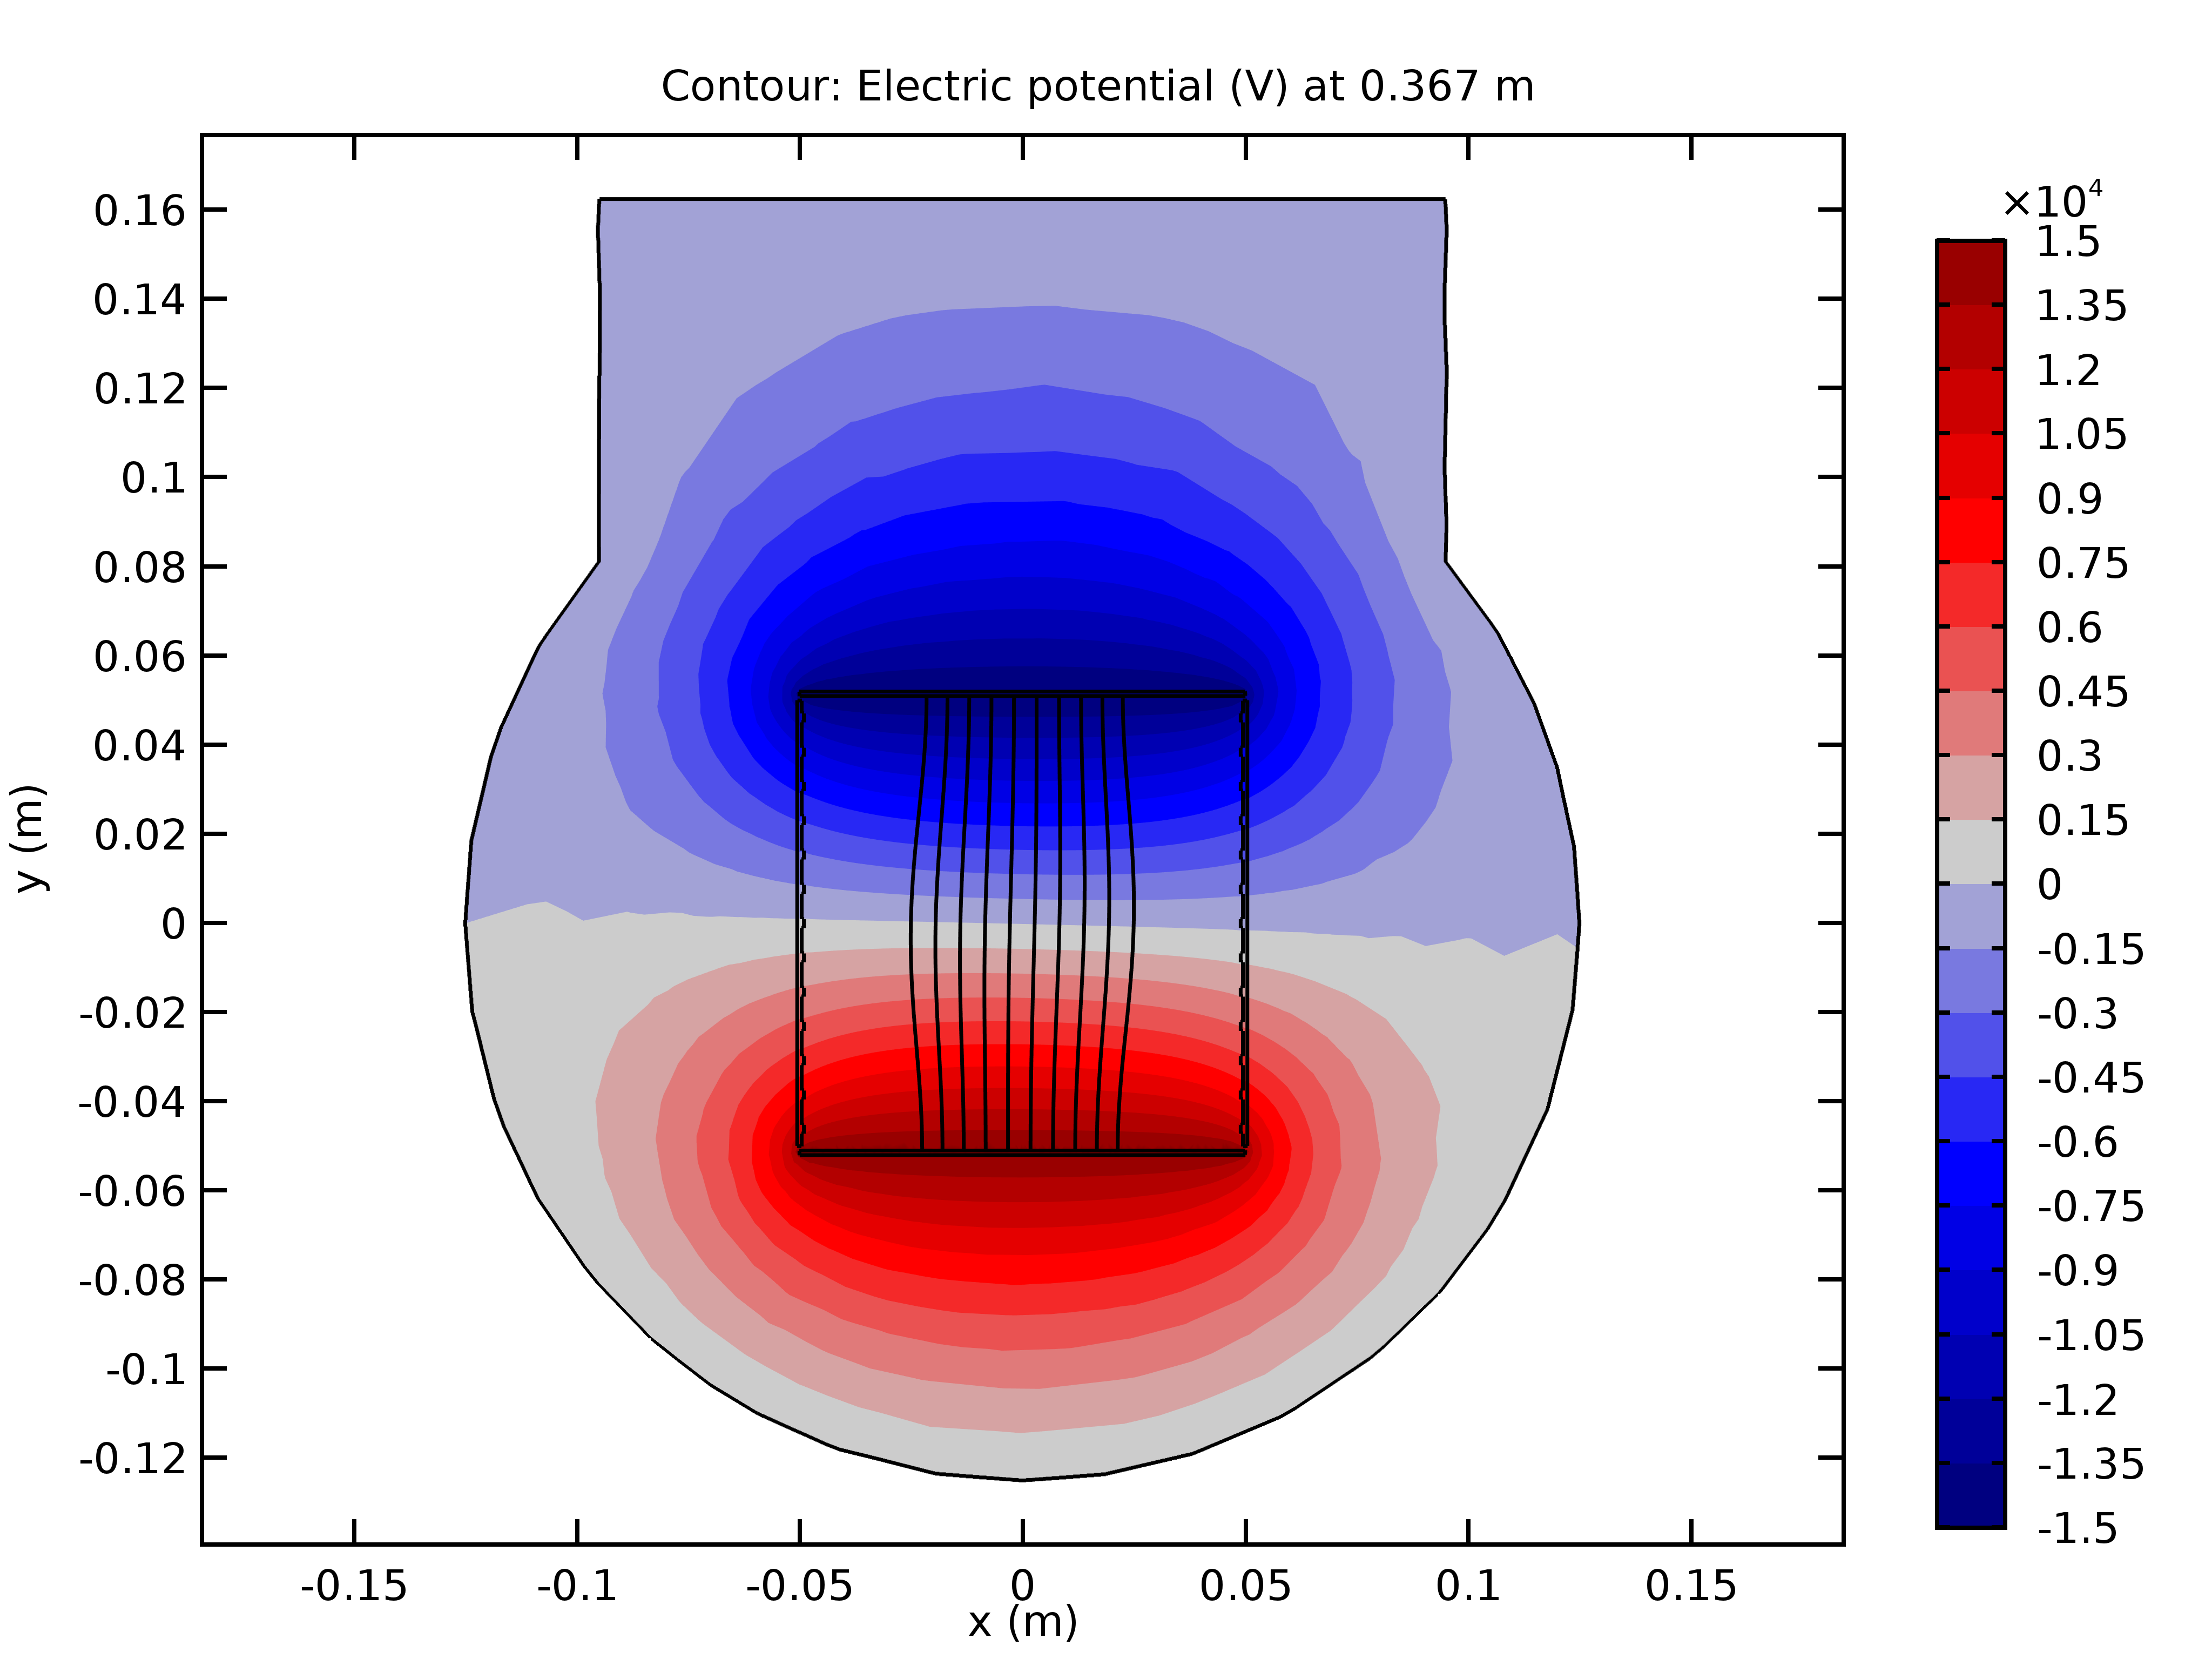
\includegraphics[width=\textwidth]{03_Prototype/figures/fig021_image_asym_sym_b.png}
		\caption{Symmetric configuration.}
		\label{chap3:asym_sym_b}
	\end{subfigure}
	~
	\begin{subfigure}{0.5\textwidth}
		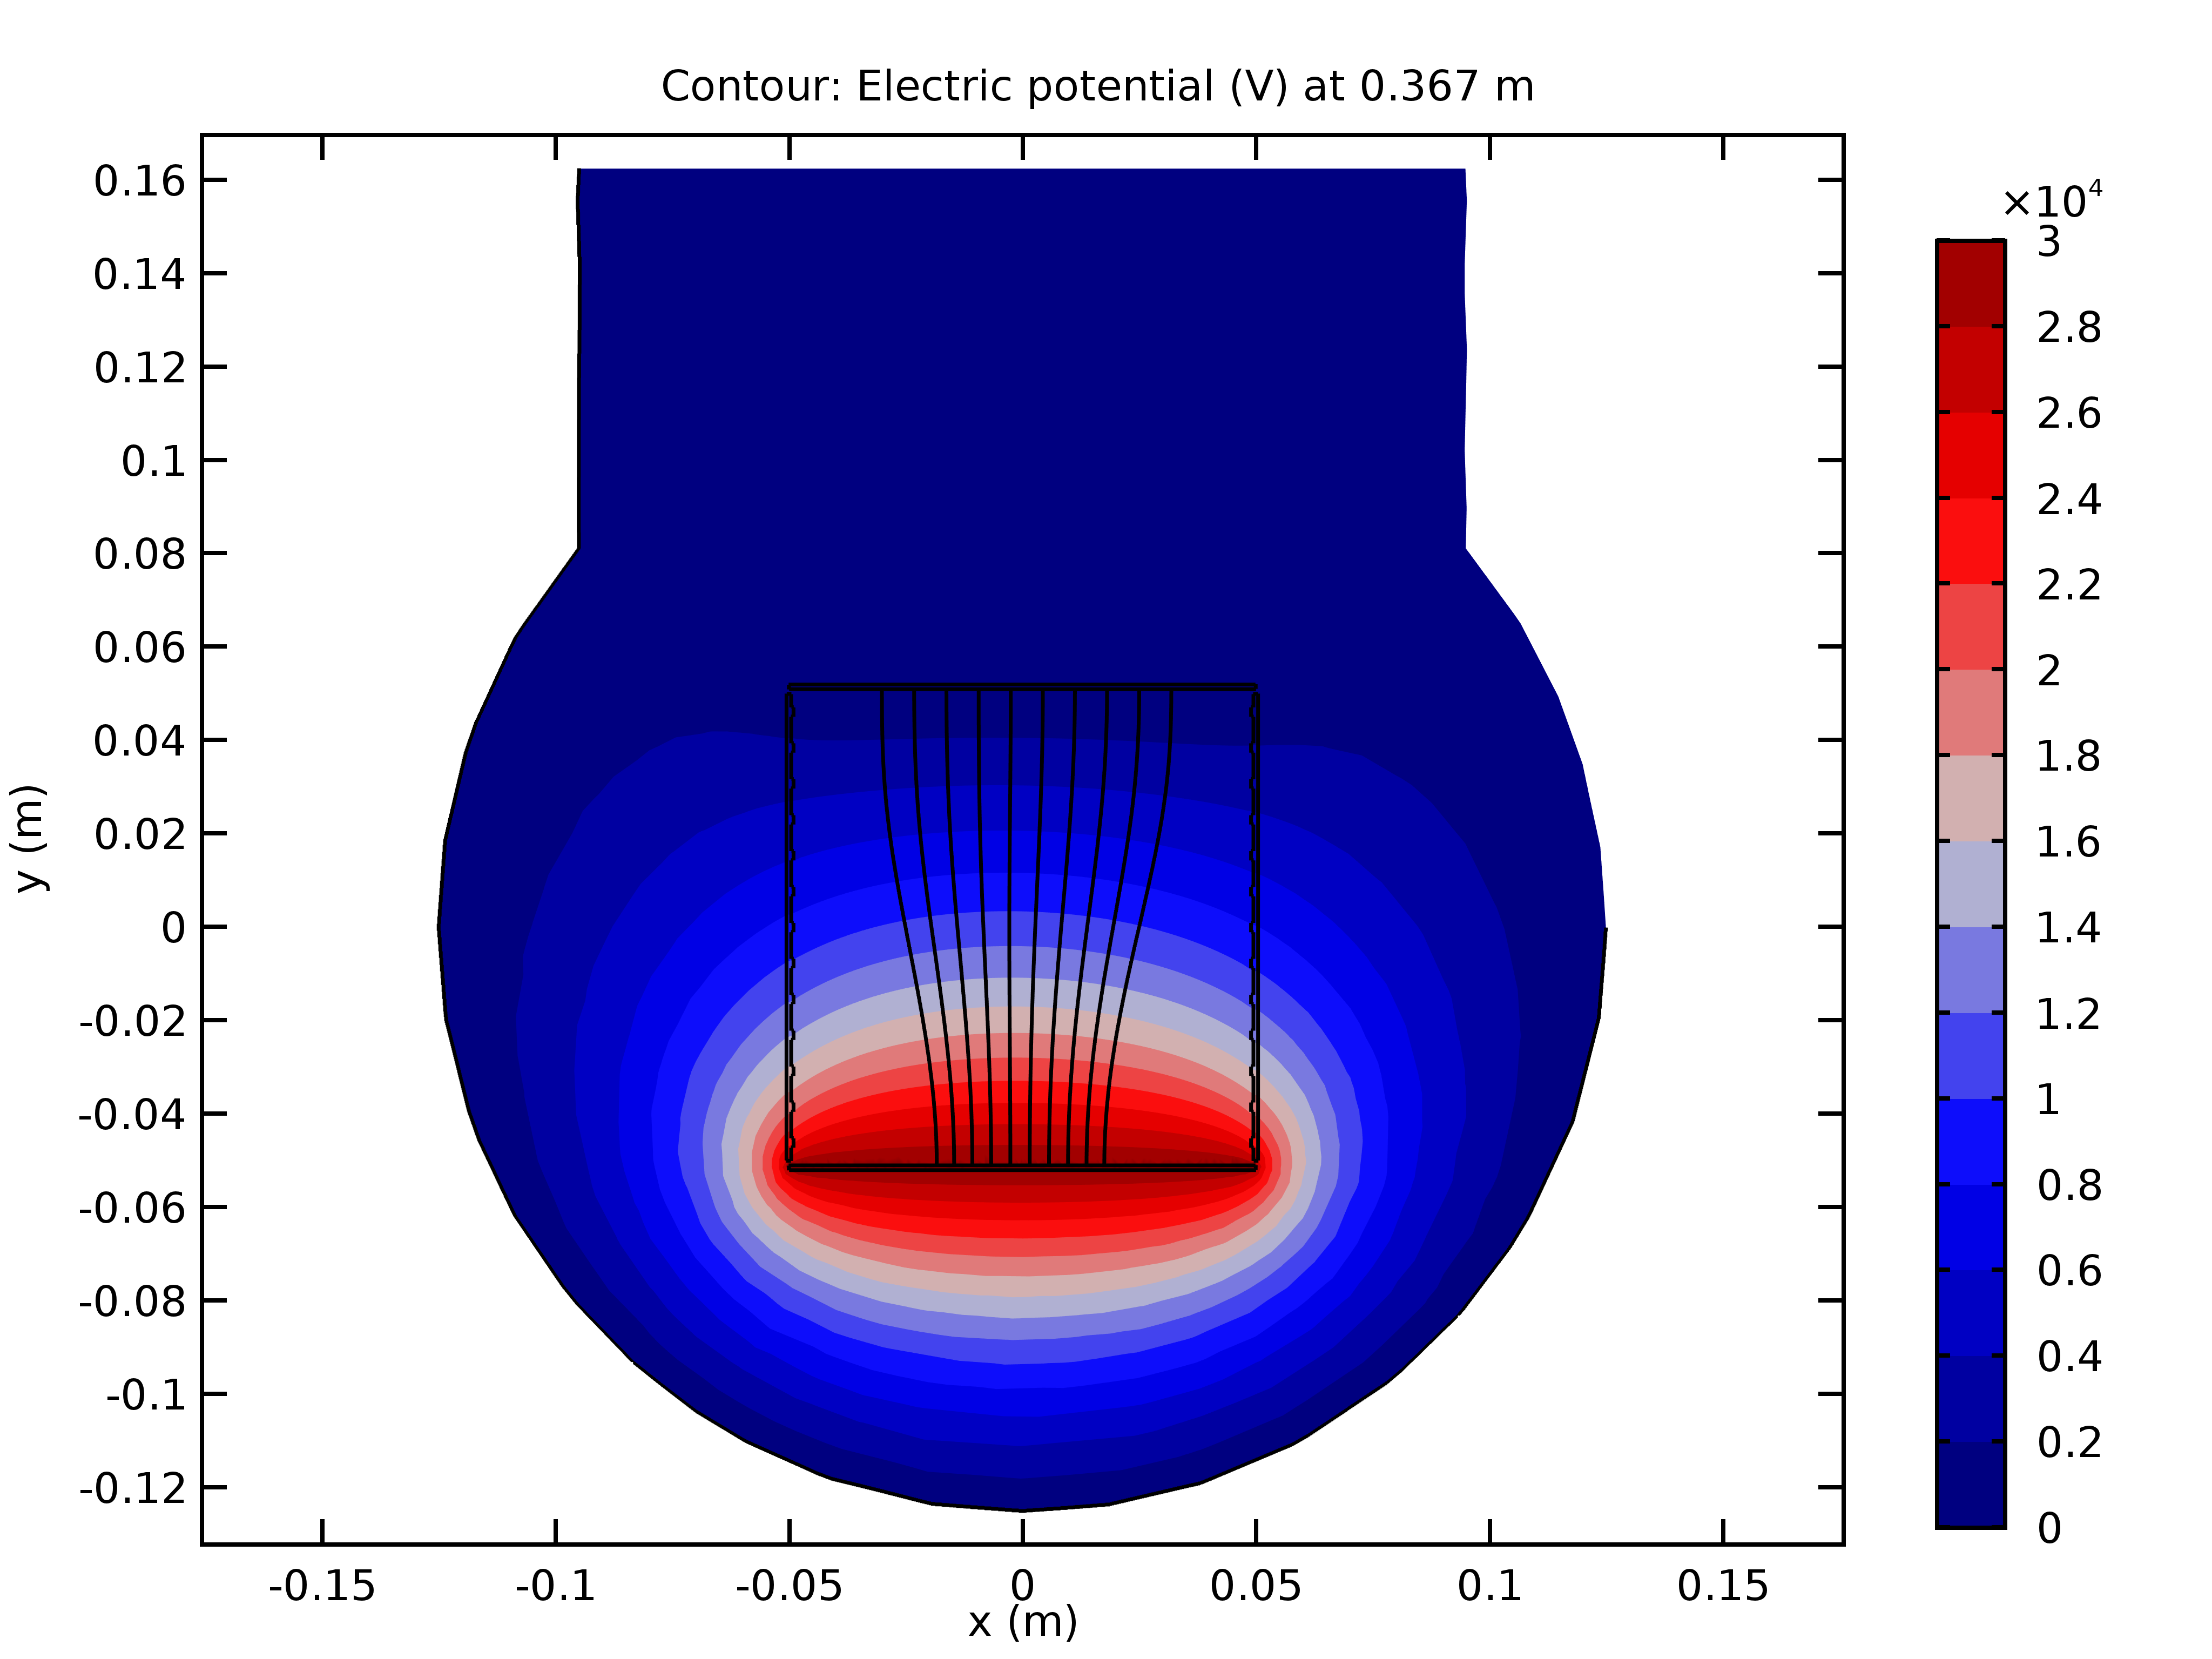
\includegraphics[width=\textwidth]{03_Prototype/figures/fig021_image_asym_sym_a.png}
		\caption{Asymmetric configuration.}
		\label{chap3:asym_sym_a}
	\end{subfigure}
	\caption[Comparison between symmetric and asymmetric configuration]{Comparison between symmetric and asymmetric configuration.}
	\label{chap3:asym_sym}
\end{figure}


	In this configuration (Fig. \ref{chap3:asym_sym_b}), the field focuses the particles in the transverse plane but also in the longitudinal plane. This explains why the particle number on the readout is higher than the expected number. In symmetric, only the transverse plane should be corrected.

	In asymmetric configuration (Fig. \ref{chap3:asym_sym_a}), the field is defocusing in the transverse plane, but also in the  longitudinal one. The projection of the beam will be much broader than expected and many particles are lost during the particle drifts. Therefore, the electric field must be improved in both planes.


	\subsection{IPM cross-interaction}

	The IPMs are in close proximity in order to measure the two transversal  directions. This proximity leads to a coupling effect between the two IPMs due to fringe fields. Moreover, the uniformity of the electric field is strongly related to the geometry that encloses the IPMs. The LWU walls itself are at ground level, hence the uniformity of the IPMs is dependant of their position in the LWU. This means that each IPM has to be corrected individually.

	We simulated in COMSOL different IPM configurations with or without disks at several positions. The IPMs cannot be shifted too much because the space on left is limited by the WS on left and by the LWU walls on right. So, we found out that it is much easier to use disks. Fig. \ref{chap3:IPM_disk} shows the influence of disk on the electrical field.

	\begin{figure}[!ht]
	\centering
	\begin{subfigure}{0.7\textwidth}
		\includesvg[width=\textwidth]{03_Prototype/figures/fig022_2IPM_ASYM_NODISK_NODEG_a}
		\caption[]{Electrical field without disk.}
		\label{chap3:no_disk}
	\end{subfigure}

	\begin{subfigure}{0.7\textwidth}
		\centering
		\includesvg[width=\textwidth]{03_Prototype/figures/fig022_2IPM_ASYM_DISK_NODEG_c}
		\caption{Electrical field with disks.}
		\label{chap3:disks}
	\end{subfigure}
	\caption[Influence of shielding disks on the IPM electric field]{Influence of shielding disks on the IPM electric field along the LWU.}
	\label{chap3:IPM_disk}
\end{figure}


	The quadratic mean is plotted for each electrical component in the middle of the IPM, as described in section \ref{}. A strong overlap occurs when no disk are between the two IPMs. When disks are enabled, the fields are constrained within the space in two disks and the cross interaction effect is less important. On the other hand, the field variations are sharper in this area, so the longitudinal field component is worse with disks. One can see that the field shape is same in both IPMs because they are independant to the LWU geometry. This is quite useful because the same corrections can be applied to the two IPMs and it simplifies the optimization of field correctors.

	\clearpage
	\subsection{Field corrections}
	\begin{wrapfigure}{r}{0.45\textwidth}
	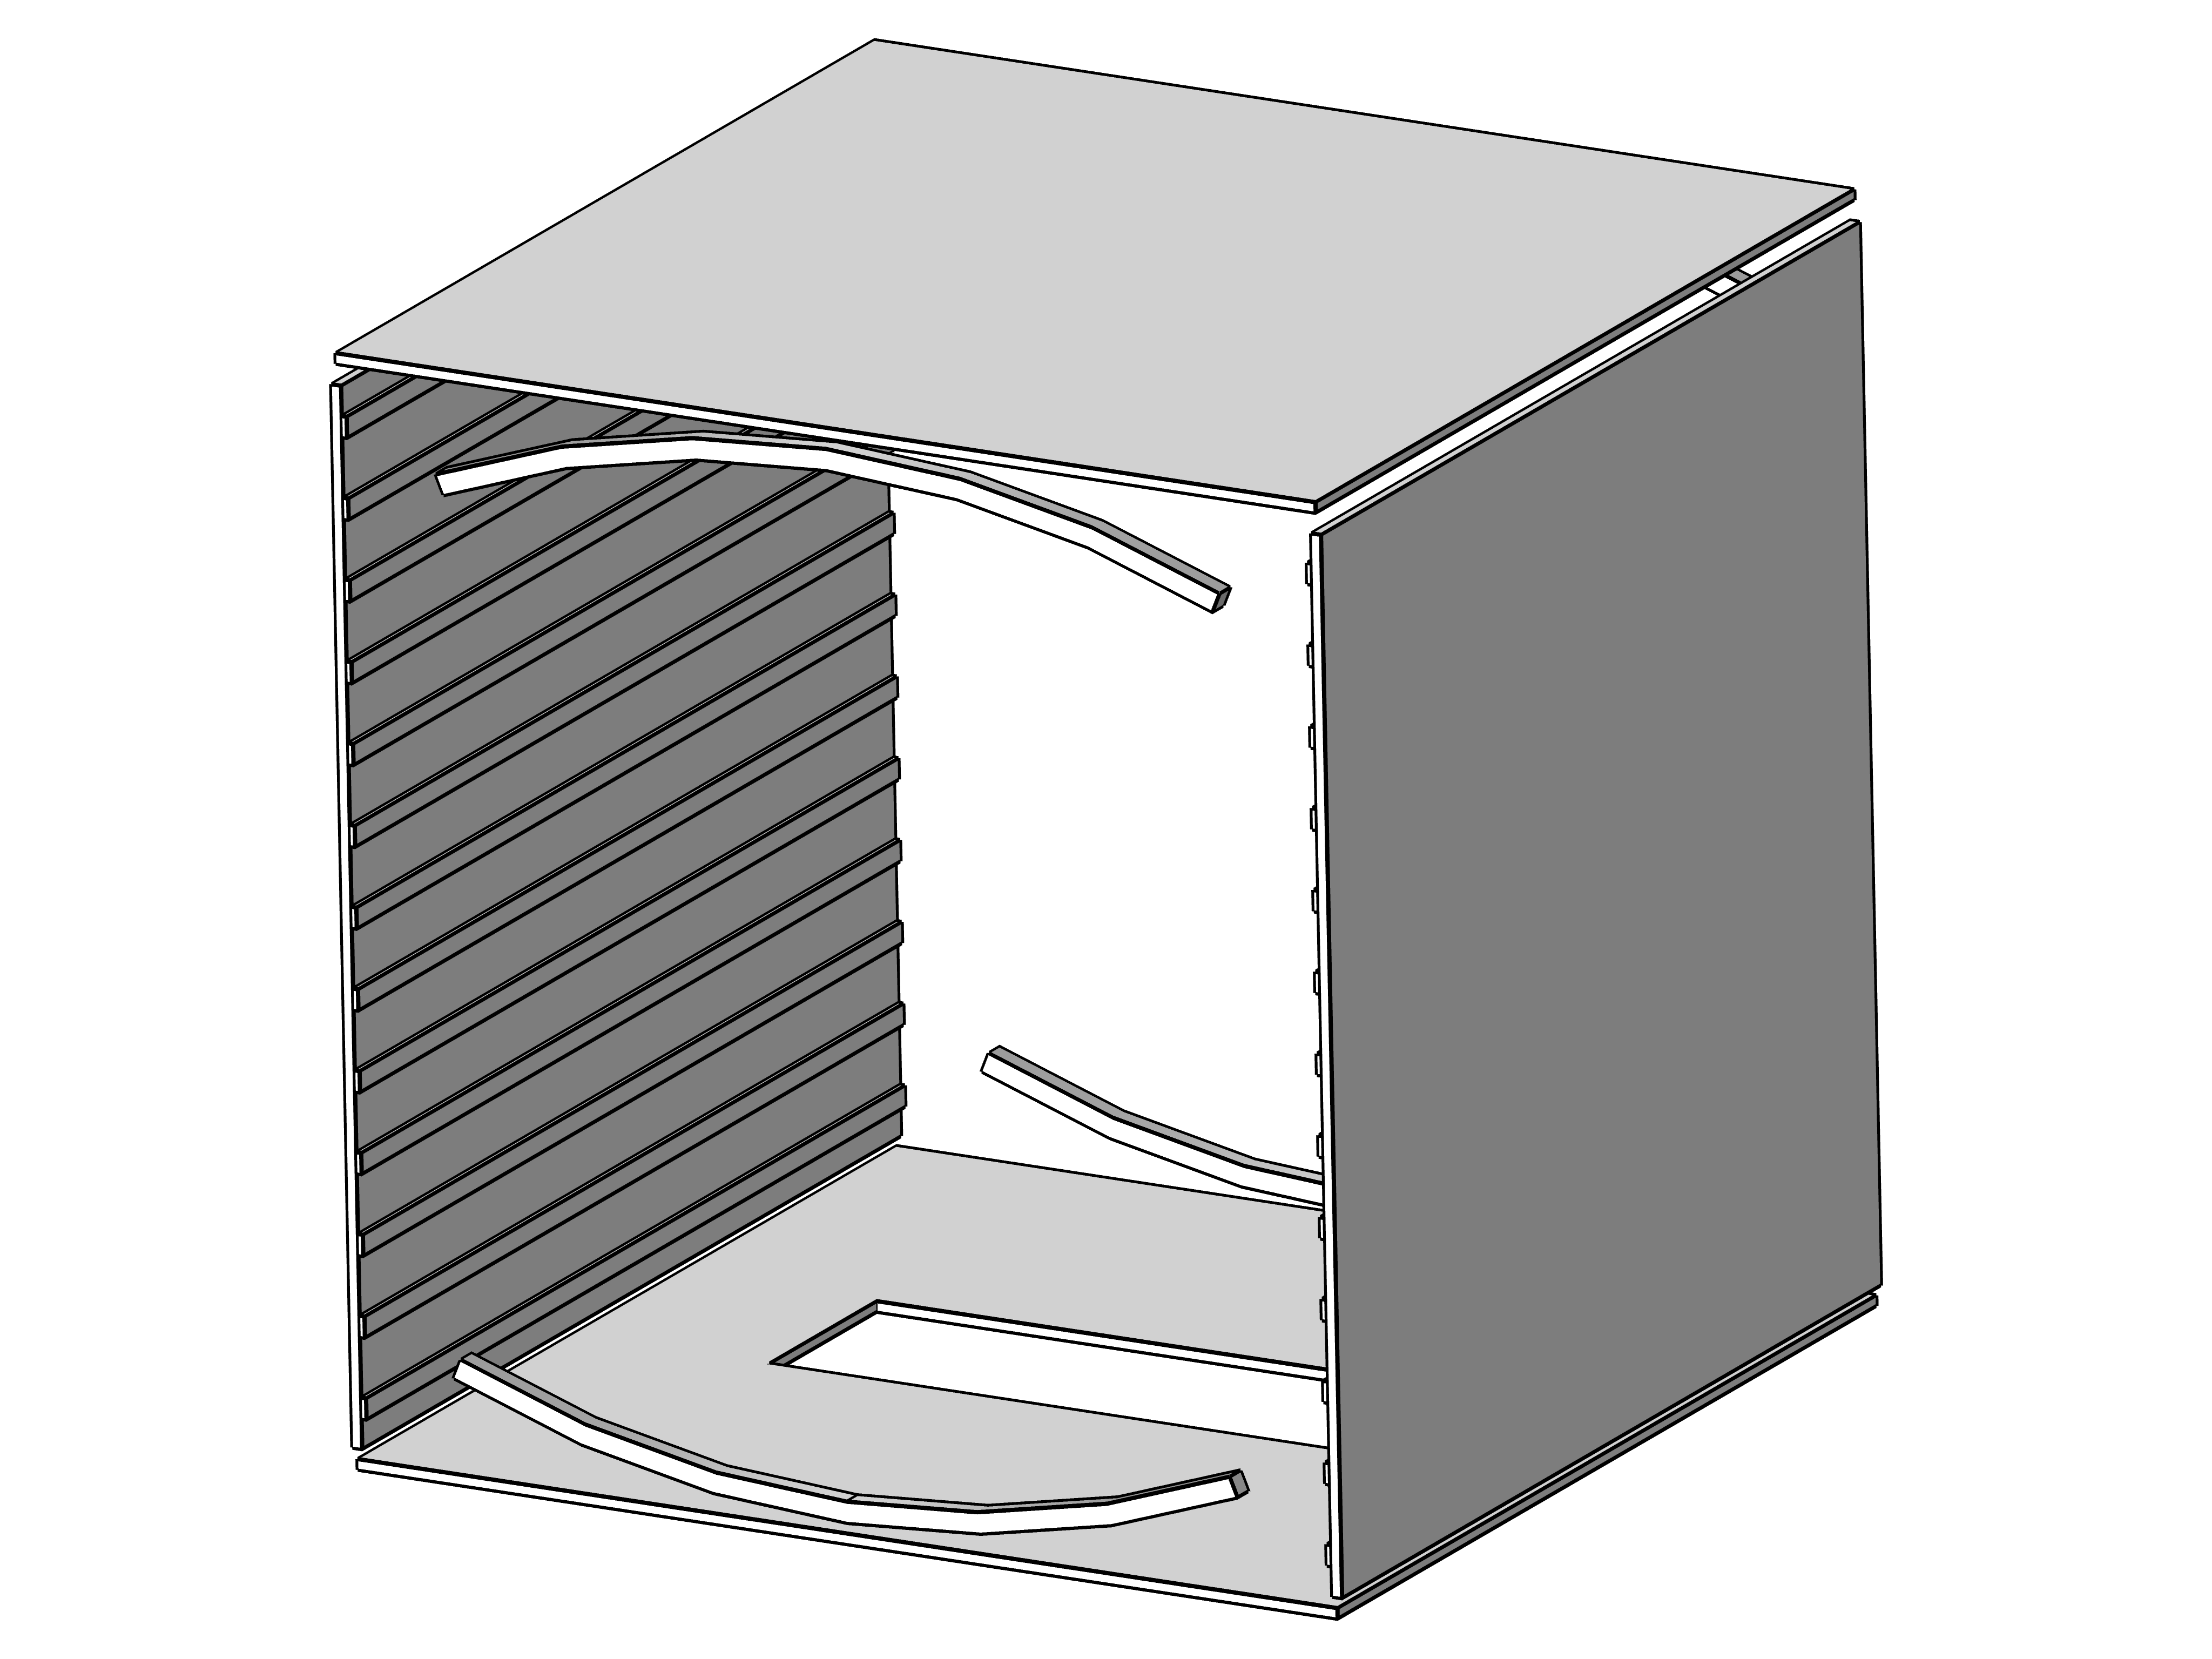
\includegraphics[width=0.45\textwidth]{03_Prototype/figures/fig026_IPM_COMSOL.png}
	\caption[IPM geometry in COMSOL]{IPM geometry in COMSOL.}
	\label{chap3:IPM_COMSOL}
\end{wrapfigure}

	The electric field will be improved by means of field correctors (also called field degraders) and curved electrodes. The Fig. \ref{chap3:IPM_COMSOL} shows the COMSOL an example of IPM that has been simulated. One can see the degraders on each side and the curved electrodes at the top and bottom of each of the IPM.

	The field correctors will constrain the electric potential at a certain value on the side of the IPM. Thus, the iso-potential will be more flat in the IPM, so the field be more uniform. In practice, field degraders are just conductive pieces connected to a voltage source. One can directly connect them to power supplies. This method allows to tune finely the potential on the electrodes.
	On the other hand, it requires HV feedthroughs for each electric potential. Unfortunately, we cannot do this way since the available space on the IPM flange is restricted. We will use directly the existing high voltages to feed a resistor bridge as shown in Fig. \ref{chap3:resistor_chain}. The potential at each field corrector is simply given by the Ohm law:
	\begin{equation}
		V_{i} = \frac{\sum_{k = 1}^{i} R_{k}}{\sum_{j = 1}^{N} R_{j}}V_{HV}
	\end{equation}

	\begin{wrapfigure}{l}{0.3\textwidth}
	\begin{center}
		\begin{tikzpicture}[scale=0.8,transform shape,american voltages]
			\draw (0,0) node[label={above:HV}] {} to [short, *-] (2,0)
			to [R, l_=$R_1$] (2,2)
			to [R, l_=$R_2$, *-] (2,4);
			\draw (0, 9) node[label={above:HV}] {} to [short, *-] (2,9)
			to [R, l_=$R_{N}$] (2,7)
			to [R, l_=$R_{N-1}$, *-] (2,5)
			(2,4.5) node[] {...};
		\end{tikzpicture}
	\end{center}
	\caption[Resistor chain]{Resistor chain.}
	\label{chap3:resistor_chain}
\end{wrapfigure}


	The method is straightforward to implement but has some drawbacks. The choice of resistor is limited since all resistance values are not available commercially \cite{Vishay2012}. Thus, all correction possibilities are not possible. The use of resistor in a vacuum is not really recommended since it often require welding. Also, the resistor should should sustain the radiative environment. Moreover, if one of the resistance is damaged the entire bridge is affected.

	We decided to use $13$ degraders on each side of the IPM. A degrader is $2\,\mathrm{mm}$ width and $100\,\mathrm{mm}$ long (in longitudinal direction) and regularly spaced by $7.5\,\mathrm{mm}$ from the others. The $7^{th}$ degrader is located in the middle plane of the IPM.

	The electric potential value, which gives the best uniformity, is computed with COMSOL for each degrader. The resistor chain is determined from these values with respect to the equation. For each corrector, two commercial off-the-shelf (COTS) resistors are mounted in series allowing values close as possible to the optimal one. Resistors are selected within $\mathrm{M\Omega}$ range reducing the power consumption of power supplies. The field simulation is recomputed with the real resistor and potential values.

	In the case of the symmetrical IPM, only the first $6$ degraders must be calculated since the $7^{th}$ is grounded and the last $6$ potentials are just at opposite value due to symmetry. The voltage and resistor values of the degrader chain for symmetric IPM are tabulated in the Table \ref{chap3:resistor_sym}.

	\begin{table}[ht]
	\centering
	\caption[Description of the resistor chain for the field degraders in the symmetric IPM]
	{Description of the resistor chain for the field degraders in the symmetric IPM.}
	\label{chap3:resistor_sym}
	\begin{tabular}{lllllllll}
		\toprule
		                                & 1  & 2     & 3      & 4    & 5      & 6     & 7    &    \\
		\midrule
		%Voltage (\(\mathrm{kV}\))       & 15 & 13.57 & 11.32  & 8.72  & 6.52   & 4.31  & 2.16 & 0  \\
		%Resistor (\(\mathrm{M}\Omega\)) &    & 13.24 & 20.83  & 24.07 & 20.37  & 20.46 & 19.9 & 20 \\
		Resistor (\(\mathrm{M}\Omega\)) &    & 13.4  & 20.715 & 24.3 & 20.332 & 20.51 & 20   & 20 \\
		Voltage (\(\mathrm{kV}\))       & 15 & 13.56 & 11.32  & 8.71 & 6.52   & 4.31  & 2.15 & 0  \\
		\bottomrule
	\end{tabular}
\end{table}

	A particle tracking was performed with the real corrected field and the results are shown in Fig. \ref{chap3:SymTransversalProfile}. One see that, even without correction, the symmetrical IPM gives fairly good results. The focusing effect, shown in the previous section, is visible and explain why there is more particle on readout than expected. When the field corrector are enabled, the profile is extremely well reconstructed with an error of less than $0.2\,\mathrm{\%}$.  This matches with the requirements of ESS on the profile error.

	\begin{figure}[!h]
	\begin{center}
		\includesvg[width=\textwidth]{03_Prototype/figures/fig023_SymTransversalProfile}
	\end{center}
	\caption[Particle tracking for real symmetric field configuration with and without configuration]{Particle tracking for real symmetric field configuration with and without configuration (degraders and disks). Beam is assumed to be gaussian with a size $\sigma_{beam}=3\,\mathrm{mm}$ [Image à refaire]}
	\label{chap3:SymTransversalProfile}
\end{figure}


	For the asymmetric IPM, we proceeded in the same way. In this case, the resistor chain must be evaluated as well as the two curved electrodes. The Table \ref{chap3:resistor_asym}. gives the values of resistances and potentials in the case of the asymmetric IPM.

	\begin{table}[ht]
  \noindent
  \caption[Description of the resistor chain for the field degraders and curved electrodes in the asymmetric IPM]
  {Description of the resistor chain for the field degraders and curved electrodes in the asymmetric IPM. [A finir je dois remplir avec les bonnes valeurs]}
  \label{chap3:resistor_asym}
  \begin{tabular}{llllllllll}
    \toprule
                                    & Curved &      & HT    &      & 1     &      & 2    &      & 3    \\
    \midrule
    Resistor (\(\mathrm{M}\Omega\)) &        & 20.5 &       & 17.2 &       & 15.5 &      & 22.2        \\
    Voltage (\(\mathrm{kV}\))       & 30     &      & 27.63 &      & 25.64 &      & 23.85 &      & 21.29 \\
    \bottomrule
  \end{tabular}
  \\
  \medskip
  \begin{tabular}{lllllllllll}
    \toprule
                           &      & 4  &      & 5  &    & 6  &      & 7  &      & 8  \\
    \midrule
    Resistor (\(\mathrm{M}\Omega\)) & 24.1 &    & 19.5 &    & 20 &    & 19.5 &    & 13.5      \\
    Voltage (\(\mathrm{kV}\))       &      & 18.5 &      & 16.25 &    & 13.94 &      & 11.69 &      & 10.13 \\
    \bottomrule
  \end{tabular}
  \\
  \medskip
  \begin{tabular}{lllllllllll}
    \toprule
                           &    & 9  &      & 10 &      & 11 &       & 12 &      & 13 \\
    \midrule
    Resistor (\(\mathrm{M}\Omega\)) & 16 &    & 17.2 &    & 13.4 &    & 18.51 &    & 13.5      \\
    Voltage (\(\mathrm{kV}\))       &    & 8.28 &      & 6.3 &      & 4.74 &       & 2.6 &      & 1.05 \\
    \bottomrule
  \end{tabular}
  \\
  \medskip
  \begin{tabular}{llll}
    \toprule
                           &     & Gnd & Curved \\
    \midrule
    Resistor (\(\mathrm{M}\Omega\)) & 9.1 &     &        \\
    Voltage (\(\mathrm{kV}\))       &     & 0  & 2850      \\
    \bottomrule
  \end{tabular}

\end{table}

	The results of particle tracking, for the asymmetric case, are shown in Fig. \ref{chap3:AsymTransversalProfile}. The asymmetric field defocuses particle in both directions without corrections. So the profile is wider and some particles do not even reach the readout. The shift in position is due to the cross interaction between the two IPMs. When corrections are enabled, the transverse profile is much better: the error on the profile is only $X\,\mathrm{\%}$. The position is also corrected and no shift appears. However, the correction on the longitudinal field is not as good and particles are still lost during the drift: only $X\,\mathrm{\%}$ of the particles will reach the readout.

	\begin{figure}[!h]
	\begin{center}
		\includesvg[width=\textwidth]{03_Prototype/figures/fig025_AsymTransversalProfile}
	\end{center}
	\caption[Particle tracking for real asymmetric field configuration with and without configuration]{Particle tracking for real asymmetric field configuration with and without configuration (degraders and disks). Beam is assumed to be gaussian with a size $\sigma_{beam}=3\,\mathrm{mm}$.}
	\label{chap3:AsymTransversalProfile}
\end{figure}


	\subsection{Grid}
	\label{chap3:sec:grid}
	As shown in the Fig. \ref{chap3:IPM_COMSOL}, the readout electrode is not completely fill: a rectangular slit allows the ions or electrons to move toward the readout system. This slit is relatively big ($2\times5\,\mathrm{cm^{2}}$) with respect to the electrode dimensions ($10\times10\,\mathrm{cm^{2}}$), so it affects the electric field uniformity. A wire mesh can easily overcome this problem, indeed in the close proximity of a mesh, the field is not very straight, but at farther distances the field becomes constant. The mesh allows to have always the same field uniformity in the IPM whatever the readout used. On the other hand, it is obstacle for the incident particles, therefore the grid must be choose carefully.

	Actually, many of our colleagues are involved in the development of gaseous detectors. So we have access to many type of mesh. We started with a stainless steel mesh (?) with a inner pitch of $450\,\mathrm{\mu m}$ and a wire size of $50\,\mathrm{\mu m}$, so the optical transparency is about $90\,\mathrm{\%}$. The thickness is about $XX\,\mathrm{\mu m}$. A first approximation can be made with the Fourier series of the electric potential as proposed by Feynman \cite{feynman2011feynman}:
	\begin{equation}
		V(x,y)= \sum^{\infty}_{n=0} A_{n} \cdot cos(-\frac{2\pi n x}{\lambda}) \cdot exp(-\frac{2\pi n y}{\lambda})
	\end{equation}

	In this case the grid is regularly spaced in $x$ direction by a step $\lambda$. If we are at $k \cdot \lambda$ away from the grid the first harmonic is attenuated by a factor $e^{-2\pi k}$. This tendency can be easily confirm with FEM or BEM method. The Fig. \ref{chap3:Grid} shows the electrical potential close to the mesh for two different field configurations. One can see that the field is almost constant in less than $1\,\mathrm{mm}$ distance from the mesh. So there will be no problem for using this grid.

	\begin{figure}[!ht]
	\centering
	\begin{subfigure}{\textwidth}
		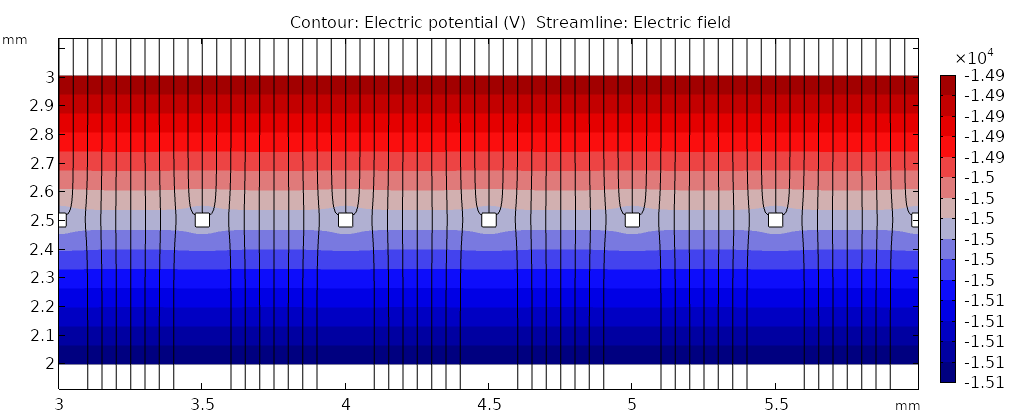
\includegraphics[width=\textwidth]{03_Prototype/figures/fig027_Grid1.png}
		\caption[]{Configuration 1: The field is constant (up: \(3\,\mathrm{kV/cm}\); down: \(3\,\mathrm{kV/cm}\)). The mesh transmission is close to the optical transparency.}
		\label{chap3:Grid1}
	\end{subfigure}

	\begin{subfigure}{\textwidth}
		\centering
		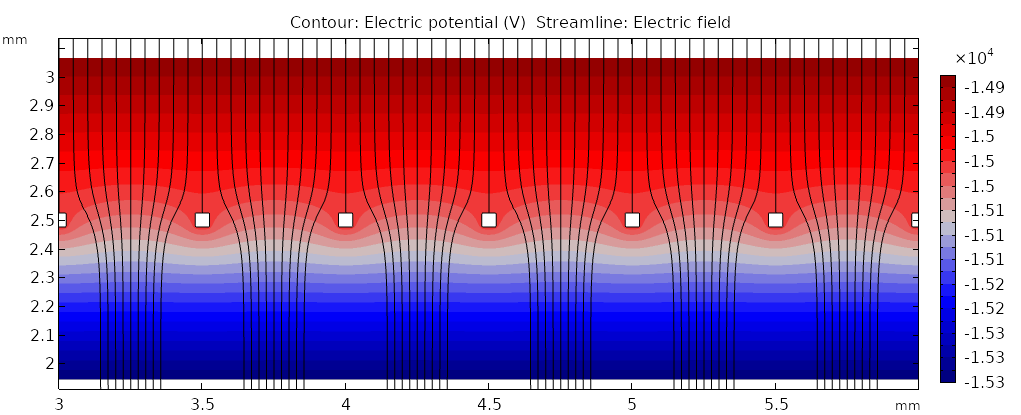
\includegraphics[width=\textwidth]{03_Prototype/figures/fig027_Grid2.png}
		\caption[]{Configuration 1: The field is higher below the grid (up: \(3\,\mathrm{kV/cm}\); down: \(6\,\mathrm{kV/cm}\)). The mesh transmission is higher than the optical transparency.}
		\label{chap3:Grid2}
	\end{subfigure}
	\caption[Electrical simulations of a \(50/450\,\mathrm{\mu m}\) grid]{Electrical simulations of a \(50/450\,\mathrm{\mu m}\) grid. Two different field configurations were simulated. Both shows that the electrical field becomes uniform few mm away from grid. However the particle transmission differs due different ratios of the electric fields imposed in the two regions.}
	\label{chap3:Grid}
\end{figure}


	The grid is an obstacle for the incoming particles, and the number of stopped particles is directly related to the optical transparency of the grid. However it is possible to improve the transmission by increasing the field on one sides of the grid. A simple analytical model has been demonstrated in the case of wire grids \cite{Bunemann1949}. We assume that our grid follows this model\footnote{This is not really true since our mesh is not made of cylindric wires.}:
	\begin{equation}
		\frac{E_{r}}{E_{d}} \geq \frac{1+\frac{2 \pi r}{\lambda}}{1-\frac{2 \pi r}{\lambda}}
	\end{equation}
	Where, $E_{r}$ is the field on the readout region, $E_{d}$ is the field on the drift region and $r$ the wire diameter. For our mesh configuration the ratio $\frac{E_{r}}{E_{d}}$ must be higher than $4.38$.
	An example is given in Fig. \ref{chap3:Grid}. The top figure shows a case where $E_{r}=E_{d}$. The field lines may be stop by the mesh wires. In the bottom figure, $E_{r}=2 \cdot E_{d}$, now the field line are attracted into the readout region due to the field difference.

	The grid can be polarized in order to use it as Frish grid. For some readout, it allows to get rid of certain signal contributions. More details will be given in section \ref{chap3:ramo} of this chapter.

	Finally, the grid may be also used to shield the readouts against possible electromagnetic noises created by all the radio-frequency devices. The effectiveness of the grid is clear. The wavelengths for the two ESS frequencies\footnote{We only considered the first harmonic} are respectively $80\,\mathrm{cm}$ and $40\,\mathrm{cm}$. The pitch of our grid is far less than theses wavelengths.

	\subsection{Summary}

	\section{Initial momentum}
  So far, we assumed that the ions and/or electrons were created without initial velocity ie at rest in a pure electrical field. In this case, electrons and ions give same results and the value of extraction field does not matter. In reality, these particles have a non-negligible initial speed and may be affected by parasitic electromagnetic fields. This can greatly affect the profile, thus the extraction field must be increased in order to minimize the distortion. In the following sections, we will try quantify these effects to determine the nominal value of the extraction field. 
  %The second limitation concerns possible \acrshort{hv} breakdowns. In very high vacuum a distance of some millimeter is sufficient to isolate several tens of kilovolts. However, the breakdowns are also strongly influenced by the surface states of the electrodes, the composition of the vacuum and the presence of leakage current \cite{Latham1995}. Hence, we should keep a standoff distance between the electrode and the vacuum vessel (less than 1kV/cm between the IPMs and LWU).

	\subsection{Thermal distribution}
	A first approximation of the initial speed of ions can be done thanks to the distribution of Maxwell-Boltzmann. The distribution of the speeds with respect to the particle mass and the temperature is given by the following equation:

	\begin{equation}
		F(\boldsymbol{v}) = \left(\frac{m_{part}}{2 \pi k_{b} T}\right)^{\frac{3}{2}}\exp\left(-\frac{m_{part}\boldsymbol{v}^{2}}{2 k_{b} T}\right)
	\end{equation}
	% \begin{wrapfigure}{r}{0.5\textwidth}
% 	\includesvg[width=0.5\textwidth]{03_Prototype/figures/fig013_maxwell_gas2}
% 	\caption[Maxwell-Boltzmann distribution for some species of ESS residual gas]{Maxwell-Boltzmann distribution for some species of ESS residual gas.}
% 	\label{chap3:maxwell_gas}
% \end{wrapfigure}
\begin{figure}[!ht]
	\centering
	\includesvg[width=0.7\textwidth]{03_Prototype/figures/fig013_maxwell_gas2}
	\caption[Maxwell-Boltzmann distribution for some species of ESS residual gas]{Maxwell-Boltzmann distribution for some species of ESS residual gas.}
	\label{chap3:maxwell_gas}
\end{figure}
	Where, $k_{b}$ is Boltzmann constant , $T$ the temperature, $\boldsymbol{v}$ is the speed vector of the considered particle and $m_{part}$ its mass. Maxwell-Boltzmann distribution works well for perfect gases at low densities. We assumed that is true for the ESS residual gas. The speed is uniformly distributed along the all direction ($4\pi$).

	The Fig. \ref{chap3:maxwell_gas} shows the normalized distributions for some of the molecules present in the ESS residual gas. One can see directly that the speed of the fastest ion is below $5000\,\mathrm{m/s}$. A field of few hundred volts per centimeter is more than enough to compensate this effect. It gives no significant difference during the particle tracking. So, we can completely neglect the thermal motion for ions.

  \subsection{Ionization energy distribution}
  
  \begin{figure}[!ht]
	\begin{subfigure}{0.5\textwidth}
		\includesvg[width=\textwidth]{03_Prototype/figures/fig028_garfield_energy.svg}
		\caption{Electron energy distribution.}
		\label{}
	\end{subfigure}
	~
	\begin{subfigure}{0.5\textwidth}
		\includesvg[width=\textwidth]{03_Prototype/figures/fig028_garfieldangle_2.svg}
		\caption{Electron emission angle distribution}
		\label{}
	\end{subfigure}
	\caption[Energy and emission angle of the ionized electrons]{Energy and emission angle of the ionized electrons.}
	\label{chap3:garfieldangle}
\end{figure}

	\section{Space charge effect}
	\subsection{Lorentz transformation of electromagnetic fields}
	\subsection{ESS/CEA Space Charge algorithm}
	\subsection{Results/Comparisons/???}
	\section{Readout systems}
	% TODO: A améliorer
	The trajectory of particles is now defined. There remains only the crucial step of the detection of these particles. We want to collect a small number of positive or negative charged particles at relatively low energies. The most suitable methods are conductive floors and solid state detectors. These methods are also more or less compatible with vacuum use.

	Detection conductive strips because it is the simplest and most robust method to implement. Unfortunately, the sensitivity is quite limited and when the signal is too weak, it is necessary to add an Micro Channel Plate type amplifier. Finally, we also considered the newly developed CERN method based on semiconductor detector. In this section we present the operating principles of these three methods.

	\subsection{Ramo-Shockley theorem}
	\label{chap3:ramo}
	In particle detectors, the signal is due to the motion of charges within the detector rather than the direct collection of charge by the electrodes. This theorem has been independently demonstrated by Ramo and Schockley \cite{Ramo_1939,Shockley_1938}. The total charge induced on an electrode at a time $t$ by a $q$ charged particle can be easily determined if the particle velocity $\boldsymbol{v}$ and the weighting field $\boldsymbol{E}_{w}$ of the electrode are known:
	\begin{equation}
		i_{n}= q\boldsymbol{v} \cdot \boldsymbol{E}_{wn}
	\end{equation}
	The weighting field is virtual field calculated as follow. All charge are removed, the electrode of interest is set at 1 V while the other electrodes are at ground. This field therefore strongly depends on the electrode and detector geometry.

	Note that if two particles have the same trajectories but opposite charges, the signal will be cancel. In practice, ions and electrons go in two opposite directions in an constant electric field, so the signal adds up. However the electron is much faster, thus it create a very fast signal while the ion signal is more spread in time.

	In general to get rid of one of the components of the next signal that we want to detect ions or electrons. This is done using a so-called Frish grid, placed at a slightly different potential with respect to the reading electrodes. This grid confines the weighting fields in a restricted area and only the particles reaching this zone will induce signal. The grid must have a good transmission (as seen in section \ref{chap3:sec:grid}) it inefficiency remains low as possible \cite{Khriachkov1997,Gook2012}.


	%So if we know the trajectory of the particle it is possible to calculate the current on the electrode at each time.

	%\cite[]{Jen1941}
  \subsection{Strips based detection}
  Conductive strips is the simplest method to implement. Electrodes are etched on a PCB with a thin layer of copper. This is a direct application of Ramo-Schockley's theorem: each strip has its own sensitivity field that depends mainly on its width and its pitch with respect to the other electrodes. The signal contribution of ions or electrons can be computed for each electrodes.

  The performances of this method depend on the reading electronics. In an ideal world, a transimpedance amplifier converts and amplifies the induced current into voltage. Then, the voltage is digitized by an ADC. The gain of a transimpedance is proportional to the value of the feedback resistance.

  The reality is much more complex since the electronic elements are not perfect. The feedback resistance must be high enough for detecting small currents. But, the Johnson’s (or thermal) noise increase linearly with the resistance. At some point, the signal to noise ratio will be too low, so the signal will not be recovered. Also, a resistor is never purely resistive and has a parasitic capacitance. As will strip electrodes, PCB traces, cable and almost every component in the analog acquisition chain have parasitic impedance.

  \begin{figure}[!ht]
  \begin{center}
    \begin{tikzpicture}[scale=1,transform shape,american voltages]
      % Sensor + Cable
      \draw
      (0,0) to[isource, l_=$s$](0,3)
      to[short, -, f=$i_s(t)$] (1.5,3)
      to[C=$C_s$] (1.5,0) -- (0,0);
      \draw 
      (1.5,3) -- (3,3) to[R=$R_s$] (3,0) node[ground] {} to[short] (1.5,0);
      \draw 
      (3,3) -- (4.2,3) to[L=$L_c$] (5.2,3) to [R=$R_c$] (7.2,3) to [C,l_=$C_c$] (7.2,0) to[short] (3,0);
      
      % OPA
      \draw
      (10,2) node[op amp] (opamp) {}
      (opamp.-) |- ($(opamp.-)+(0.2,1)$) to[R=$R_f$] ($(opamp.-)+(2.2,1)$) -|
      (opamp.out)
      (opamp.-) |- ($(opamp.-)+(0.2,2.5)$) to[C=$C_{f}$] ($(opamp.-)+(2.2,2.5)$) -|
      (opamp.out)
      to[short] ($(opamp.out)+(.5,0)$) node [right] {$V_{out}$} node [ocirc] {} (opamp.+) to[short]  ($(opamp.+)-(0,.5)$) node[ground] {} (opamp.-) to[short] ($(opamp.-)-(0,0)$) |- (7.2,3);

      % Rectangle
      \draw[red, thick] (-0.5, -1) rectangle(3.9,4.)
      node[above,xshift=-2cm]{Sensor};
      \draw[blue, thick] (4.1, -1) rectangle(8.,4.)
      node[above,xshift=-2cm]{Cable};

    \end{tikzpicture}
  \end{center}
  \caption[Typical circuit of a charge amplifier with an operational amplifier]{Typical circuit of a charge amplifier with an operational amplifier. The $R_{f}$ and $C_{f}$ should chosen according to sensor characteristics. Strips sensors have low resistance but non negligible capacitance. Usually, cables are modelized by succession of LRC cells, for convenience just one cell is drawn here.}
  \label{chap3:AOPcharge}
\end{figure}



  The transimpedance amplifier is so 

  Note that the amplifier has its own characteristics that will also limit bandwidth and gain depending of amplifier architecture and technology. This topics is very wide and we just introduced the basics.

  This method can not be used when the signal is too weak with respect to the electronics. Therefore, it is necessary to find a way to amplify the primary signal.

  \subsection{Interaction of particles with low energies}
  In general, a amplification medium is used to increase the signal. In this medium, a primary particle will create many secondary particles. These secondaries will induce an higher signal on the reading electronic. This is the operating principle of gaseous and solid state detectors. Two solid state detector technologies have been forseen since the use of gas detectors is not possible here.

  We should ensure that the detection of low energy ions or electrons is possible for these detectors. The models based on the Bethe equation, presented in the section \ref{chap3:sec_particle_in_matter}, are not precise for these energies and more specific models must be used. Unfortunately, we can not explain and describe these models here. It is much easier to use existing tools for estimating the interaction of particles at low energies. These usually rely on the Monte Carlo methods and we used two different ones.

  SRIM software simulates the interaction of heavy charged particles in matter \cite{srim2013}. The user defines different layers of compounds and the properties of the incident particle in a graphical interface. Then, SRIM computes, among others, the energy depositions, the stopping range, atomic displacements, atom vacancies in the layers. 
  
  Geant4 is a software toolkit that simulates the interaction of particle in a detector \cite{Allison2006, Allison2016}. It is a popular tool for simulating detectors of nuclear or high energy physics. The user describes a detector geometry and associated materials as well as the characteristic of the primary particles. Then, the user adds physical process that will be used for each particle interaction. In our case three models are particularly interesting: the IRCU73 model (ions) the Livermore model (ions and electrons) and the Penelope model (electrons) \cite{Bimbot73,livermore97, salvat2009}. They describe the electromagnetic interaction of charged particle in matter for low energies. A simulation, that uses the previous model, has been developed from a example provided in Geant4 (TestEM11). The simulation tries to reproduce the principles of SRIM. A cube is cut into different layers and the energy loss in each layer is saved.

  \begin{figure}[!h]
	\begin{subfigure}[t]{.5\textwidth}
		\centering
		\includesvg[width=\textwidth]{03_Prototype/figures/fig004_ion_si_deposit}
		\caption[Energy deposition in a silicon layer for various ions]{Energy deposition in a silicon layer for various ions.}
		\label{chap3:ion_si_deposit}
	\end{subfigure}
	~
	\begin{subfigure}[t]{.5\textwidth}
		\centering
		\includesvg[width=\textwidth]{03_Prototype/figures/fig005_electron_si_deposit}
		\caption[Energy deposition in a silicon layer for electrons]{Energy deposition in a silicon layer for electrons.}
		\label{chap3:electron_si_deposit}
	\end{subfigure}
	\caption[Energy deposition in a silicon layer for ions and electron at low kinetic energyies]{Energy deposition in a silicon layer for ions and electron at low kinetic energyies.}
	\label{chap3:si_deposit}
\end{figure}

  
  Fig. \ref{chap3:si_deposit} shows the energy deposition for different ions (left) and electrons (right) in a silicon cube. For same energies, the electrons deposit their energies along a higher range compare to the ions. Heavy ions are completely stopped before $200\,\mathrm{nm}$ for energies below $15\,\mathrm{keV}$. We want to remind that heavy ions may represent two-thirds of the expected signal.

	\subsection{Semiconductor based detection}
	\cite[]{Cavalleri1971}
	\cite{Allison2006,Allison2016}\cite{srim2013}
	\subsection{MCP based detection}

	A MicroChannel Plate (MCP) generates electrons from incident particles \cite{Wiza1979}.
	It can be seen as a glass lead plate drilled with micro-metric tilted holes.
	A specific coating is applied on its input surface to increase secondary emissions. When a particle hits the MCP hole entrance then secondary electrons are emitted. Due to difference of potential, secondaries are drawn towards the channel output and strike hole walls again, creating more and more electrons. Then, electrons are collected on a detection plane that can be a single electrode, multiple electrodes or a phosphorus screen depending on the requirements (sensitivity, spatial and time resolution). Fig. \ref{chap3:MCPoutline} presents some schematic representations of how an MCP works.

	\begin{figure}[!ht]
	\begin{subfigure}[t]{0.5\textwidth}
		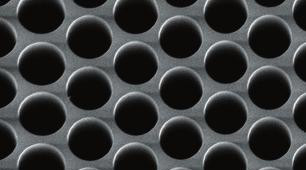
\includegraphics[width=\textwidth]{03_Prototype/figures/fig030_MCPoutline_b2.jpeg}
		\caption[SEM picture of MCP holes]{SEM picture of MCP holes \cite{HamamatsuMCP}.}
		\label{chap3:MCPholes}
	\end{subfigure}
	~
	\begin{subfigure}[t]{0.5\textwidth}
		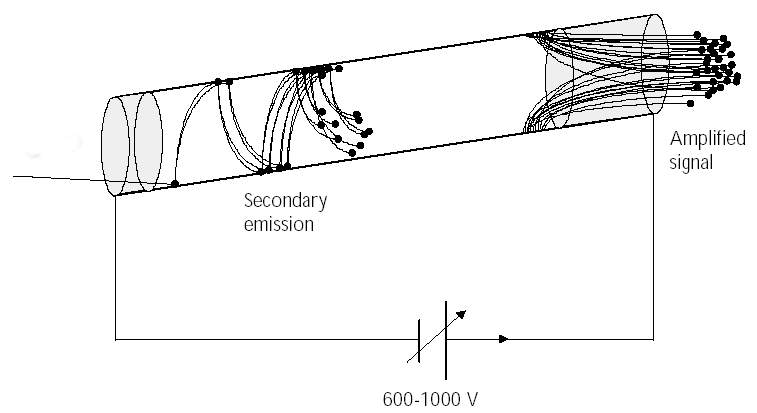
\includegraphics[width=\textwidth]{03_Prototype/figures/fig030_MCPoutline_a.png}
		\caption{Description of how an MCP amplifies incident particle.}
		\label{chap3:MCPchannel}
	\end{subfigure}
	\caption[Schematic views of how a MCP works]{Schematic views of how a MCP works.}
	\label{chap3:MCPoutline}
\end{figure}


	Gain or multiplication factor for a single MCP is about $10^{2}$ to $10^{4}$ depending on the $V_{MCP}$ voltage, usually from $600$ to $1000\,\mathrm{V}$. MCP can be stacked to increase the gain to $10^{6}$ or even more. Typical configurations are single stage, chevron stack (double stages) or Z stack (triple stages).

	Unfortunately MCPs have some drawbacks. First one is the lifetime, indeed the coating is damaged by the incident particles thus the gain is not stable and decreases over the time. Second disadvantage is the MCP gain limitation due to saturation mode. If the incident particle flux is too high then holes may be saturated, and they cannot amplify anymore. When it happens to a channel then it takes some time to recover, generating dead time.

  \section{Background signal}
  \subsection{Background from beam particles}
  \subsection{Secondary emission}

	\section{Summary}
	\label{ch3:Summary}
	[Information: textwidth in cm: \printinunitsof{cm}\prntlen{\textwidth}]

	%\begin{figure}[!ht]
	\begin{subfigure}[t]{1.\textwidth}
		\includegraphics[width=\textwidth]{example-image-a}
		\caption[]{}
		\label{}
	\end{subfigure}

	\begin{subfigure}[t]{1.\textwidth}
		\centering
		\includegraphics[width=\textwidth]{example-image-a}
		\caption{}
		\label{}
	\end{subfigure}
	\caption[]{}
	\label{chap:}
\end{figure}

	%\begin{figure}[!ht]
	\begin{subfigure}[t]{0.5\textwidth}
		\includegraphics[width=\textwidth]{example-image-a}
		\caption{}
		\label{}
	\end{subfigure}
	~
	\begin{subfigure}[t]{0.5\textwidth}
		\includegraphics[width=\textwidth]{example-image-a}
		\caption{}
		\label{}
	\end{subfigure}
	\caption[]{}
	\label{chap:}
\end{figure}

	%\begin{figure}[!ht]
	\begin{center}
		\begin{subfigure}{.5\textwidth}
			\includegraphics[width=\textwidth]{example-image-a}
			\caption{}
			\label{}
		\end{subfigure}
	\end{center}

	\begin{subfigure}{0.5\textwidth}
		\includegraphics[width=\textwidth]{example-image-a}
		\caption{}
		\label{}
	\end{subfigure}
	~
	\begin{subfigure}{0.5\textwidth}
		\includegraphics[width=\textwidth]{example-image-a}
		\caption{}
		\label{}
	\end{subfigure}
	\caption[]{}
	\label{chap:}
\end{figure}

	%\begin{figure}[!th]
	\begin{subfigure}[t]{.5\textwidth}
		\includegraphics[width=\textwidth]{example-image-a}
		\caption{}
		\label{}
	\end{subfigure}
	~
	\begin{subfigure}[t]{.5\textwidth}
		\centering
		\includegraphics[width=\textwidth]{example-image-a}
		\caption{}
		\label{}
	\end{subfigure}

	\begin{subfigure}[t]{.5\textwidth}
		\centering
		\includegraphics[width=\textwidth]{example-image-a}
		\caption{}
		\label{}
	\end{subfigure}
	~
	\begin{subfigure}[t]{.5\textwidth}
		\centering
		\includegraphics[width=\textwidth]{example-image-a}
		\caption{}
		\label{}
	\end{subfigure}
	\caption[]{}
	\label{chap:}
\end{figure}


	\cleardoublepage
	\section*{Bibliography}
	\addcontentsline{toc}{section}{Bibliography}
	\label{ch3:bib}
	\printbibliography[heading=subbibliography]

\end{refsection}